%---------------
%╔═╗╔═╗╔╦╗╦ ╦╔═╗
%╚═╗║╣  ║ ║ ║╠═╝
%╚═╝╚═╝ ╩ ╚═╝╩  
%---------------

% language setup
\newcommand{\docLanguage}{ngerman}
%\newcommand{\docLanguage}{english}

% DOCUMENT SETUP
\documentclass[12pt, oneside, a4paper, \docLanguage]{report}
\usepackage[left=3cm, 
			right=2.5cm, 
			top=2.5cm, 
			bottom=2.5cm, 
			includehead, 
			includefoot]{geometry}

% line spacing
\usepackage{setspace}
\setstretch{1,25} % 15/12 --> 1.25

% encoding setup
% T1 font encoding for languages that use a latin alphabet
\usepackage[T1]{fontenc} 

% enhanced input encoding handling - utf8 for äÄüÜöÖß...
\usepackage[utf8]{inputenc}

%de­fines Adobe Times Ro­man as de­fault text font
\usepackage{mathptmx}
\usepackage{times} % needed for acronym package

%PDF linking package
\usepackage[hidelinks]{hyperref}


% Language Setup
\usepackage[\docLanguage]{babel}
% after babel - set chapter string
\AtBeginDocument{\renewcommand{\chaptername}{}}

% language specific bibliography style
\usepackage[numbers, square]{natbib}
%\setcitestyle{square,aysep={},yysep={;}}
\usepackage[fixlanguage]{babelbib}
\selectbiblanguage{\docLanguage}
% bliographystyle setup
% babel specific: babplain, babplai3, babalpha, babunsrt, bababbrv, bababbr3
\bibliographystyle{babunsrt}


% enumeration
\usepackage{enumitem}
% tabular extension tabularx
\usepackage{tabularx}

% math packages
\usepackage{amsmath}
\usepackage{nicefrac}
\usepackage{amsthm}
\usepackage{amsbsy}
\usepackage{amssymb}
\usepackage{amsfonts}
%\usepackage{MnSymbol}


%special characters
\usepackage{amssymb}
\usepackage{upgreek,textgreek}

% acronym package
\usepackage[printonlyused, footnote]{acronym}

% breakable text in \seqsplit{}
\usepackage{seqsplit}

% \textmu
\usepackage{textcomp}

% package provides a way to compile sections of a document using the same preamble as the main document
\usepackage{subfiles}

% driver-independent color extension - used by listings,tabularx
\usepackage[usenames,dvipsnames,table,xcdraw]{xcolor}

% -- SYNTAX HIGHLIGHTING --
\usepackage{listings}
%% bash command line Syntax Highlighting
\lstdefinestyle{BASH_CMD}{ 
  columns=fullflexible,            % copy pasteable listings
  language=bash,
  basicstyle=\small\sffamily,
  basicstyle   = \small \ttfamily,
  keywordstyle = [1]\small \ttfamily,
  keywordstyle = [2]\small \ttfamily,
  commentstyle = \small \ttfamily,
  numbers=none,
  captionpos=b, 
  breaklines=true,
  numberstyle=\tiny,
  numbersep=3pt,
  frame=tlrb,
  columns=fullflexible,
  backgroundcolor=\color{white!20},
  linewidth=\linewidth,
  literate=                        % replace in code
     {Ö}{{\"O}}1 
     {Ä}{{\"A}}1 
     {Ü}{{\"U}}1 
     {ß}{{\ss}}2 
     {ü}{{\"u}}1 
     {ä}{{\"a}}1 
     {ö}{{\"o}}1 
     {â}{{\^{a}}}1 
     {Â}{{\^{A}}}1 
     {ç}{{\c{c}}}1 
     {Ç}{{\c{C}}}1 
     {ğ}{{\u{g}}}1 
     {Ğ}{{\u{G}}}1 
     {ı}{{\i}}1 
     {İ}{{\.{I}}}1 
     {ş}{{\c{s}}}1 
     {Ş}{{\c{S}}}1 
}
 % adds style BASH_CMD
%% Matlab Syntax Highlighting
\colorlet{keyword}{blue!100!black!80}
\colorlet{STD}{Lavender}
\colorlet{comment}{green!90!black!90}
\definecolor{mygreen}{rgb}{0,0.6,0}
\definecolor{mygray}{rgb}{0.5,0.5,0.5}
\definecolor{mymauve}{rgb}{0.58,0,0.82}


\lstdefinestyle{BASH_SCRIPT}{ 
  language     = bash,
  basicstyle   = \footnotesize \ttfamily,
  keywordstyle = [1]\color{keyword}\bfseries,
  keywordstyle = [2]\color{STD}\bfseries,
  commentstyle = \color{mygreen}\itshape,
  backgroundcolor=\color{white},   % choose the background color; you must add \usepackage{color} 
  columns=fullflexible,            % copy pasteable listings
                                   % or \usepackage{xcolor}
  basicstyle=\footnotesize,        % the size of the fonts that are used for the code
  breakatwhitespace=false,         % sets if automatic breaks should only happen at whitespace
  breaklines=true,                 % sets automatic line breaking
  captionpos=b,                    % sets the caption-position to bottom
  extendedchars=true,              % lets you use non-ASCII characters; for 8-bits encodings only,
                                   % does not work with UTF-8
  frame=single,                    % adds a frame around the code
  keepspaces=true,                 % keeps spaces in text, useful for keeping indentation of code
                                   % (possibly needs columns=flexible)
  numbers=left,                    % where to put the line-numbers; possible values are 
                                   % (none, left, right)
  numbersep=5pt,                   % how far the line-numbers are from the code
  numberstyle=\tiny\color{mygray}, % the style that is used for the line-numbers
  rulecolor=\color{black},         % if not set, the frame-color may be changed on line-breaks
                                   % within not-black text (e.g. comments (green here))
  showspaces=false,                % show spaces everywhere adding particular underscores; it
  	                               % overrides 'showstringspaces'
  showstringspaces=false,          % underline spaces within strings only
  showtabs=false,                  % show tabs within strings adding particular underscores
  stepnumber=1,                    % the step between two line-numbers. If it's 1, each line 
                                   % will be numbered
  stringstyle=\color{mymauve},     % string literal style
  tabsize=2,                       % sets default tabsize to 2 spaces
  title=\lstname,                  % set title name
  literate=                        % replace in code
     {Ö}{{\"O}}1 
     {Ä}{{\"A}}1 
     {Ü}{{\"U}}1 
     {ß}{{\ss}}2 
     {ü}{{\"u}}1 
     {ä}{{\"a}}1 
     {ö}{{\"o}}1 
     {â}{{\^{a}}}1 
     {Â}{{\^{A}}}1 
     {ç}{{\c{c}}}1 
     {Ç}{{\c{C}}}1 
     {ğ}{{\u{g}}}1 
     {Ğ}{{\u{G}}}1 
     {ı}{{\i}}1 
     {İ}{{\.{I}}}1 
     {ş}{{\c{s}}}1 
     {Ş}{{\c{S}}}1 
} % adds style BASH_SCRIPT
% Matlab Syntax Highlighting
\colorlet{keyword}{blue!100!black!80}
\colorlet{STD}{red}
\colorlet{comment}{green!90!black!90}
\definecolor{mygreen}{rgb}{0,0.6,0}
\definecolor{mygray}{rgb}{0.5,0.5,0.5}
\definecolor{mymauve}{rgb}{0.58,0,0.82}


\lstdefinestyle{LATEX}{ 
  language     = [LaTeX]{TeX},
  basicstyle   = \footnotesize \ttfamily,
  keywordstyle = [1]\color{keyword}\bfseries,
  keywordstyle = [2]\color{comment}\bfseries,
  commentstyle = \color{mygray}\itshape,
  %backgroundcolor=\color{white},   % choose the background color; you must add \usepackage{color} 
                                   % or \usepackage{xcolor}
  basicstyle=\footnotesize,        		   % the size of the fonts that are used for the code
  breakatwhitespace=false,         % sets if automatic breaks should only happen at whitespace
  columns=fullflexible,            % copy pasteable listings
  breaklines=true,                 % sets automatic line breaking
  captionpos=c,                    % sets the caption-position to bottom
  extendedchars=true,              % lets you use non-ASCII characters; for 8-bits encodings only,
                                   % does not work with UTF-8
  frame=single,                    % adds a frame around the code
  keepspaces=true,                 % keeps spaces in text, useful for keeping indentation of code
                                   % (possibly needs columns=flexible)
  numbers=left,                    % where to put the line-numbers; possible values are 
                                   % (none, left, right)
  numbersep=4pt,                   % how far the line-numbers are from the code
  numberstyle=\tiny\color{mygray}, % the style that is used for the line-numbers
  rulecolor=\color{black},         % if not set, the frame-color may be changed on line-breaks
                                   % within not-black text (e.g. comments (green here))
  showspaces=false,                % show spaces everywhere adding particular underscores; it
  	                               % overrides 'showstringspaces'
  showstringspaces=false,          % underline spaces within strings only
  showtabs=false,                  % show tabs within strings adding particular underscores
  stepnumber=1,                    % the step between two line-numbers. If it's 1, each line 
                                   % will be numbered
  stringstyle=\color{mymauve},     % string literal style
  tabsize=2,                       % sets default tabsize to 2 spaces
  title=\lstname,                  % set title name
  literate=                        % replace in code
     {Ö}{{\"O}}1 
     {Ä}{{\"A}}1 
     {Ü}{{\"U}}1 
     {ß}{{\ss}}2 
     {ü}{{\"u}}1 
     {ä}{{\"a}}1 
     {ö}{{\"o}}1 
     {â}{{\^{a}}}1 
     {Â}{{\^{A}}}1 
     {ç}{{\c{c}}}1 
     {Ç}{{\c{C}}}1 
     {ğ}{{\u{g}}}1 
     {Ğ}{{\u{G}}}1 
     {ı}{{\i}}1 
     {İ}{{\.{I}}}1 
     {ş}{{\c{s}}}1 
     {Ş}{{\c{S}}}1 
} % adds style LATEX
%% Matlab Syntax Highlighting
\colorlet{keyword}{blue!100!black!80}
\colorlet{STD}{Lavender}
\colorlet{comment}{green!90!black!90}
\definecolor{mygreen}{rgb}{0,0.6,0}
\definecolor{mygray}{rgb}{0.5,0.5,0.5}
\definecolor{mymauve}{rgb}{0.58,0,0.82}


\lstdefinestyle{MATLAB}{ 
  language     = Matlab,
  basicstyle   = \footnotesize \ttfamily,
  keywordstyle = [1]\color{keyword}\bfseries,
  keywordstyle = [2]\color{STD}\bfseries,
  commentstyle = \color{mygreen}\itshape,
  backgroundcolor=\color{white},   % choose the background color; you must add \usepackage{color} 
                                   % or \usepackage{xcolor}
  basicstyle=\footnotesize,        % the size of the fonts that are used for the code
  breakatwhitespace=false,         % sets if automatic breaks should only happen at whitespace
  columns=fullflexible,            % copy pasteable listings
  breaklines=false,                % sets automatic line breaking
  captionpos=c,                    % sets the caption-position to bottom
  extendedchars=true,              % lets you use non-ASCII characters; for 8-bits encodings only,
                                   % does not work with UTF-8
  frame=single,                    % adds a frame around the code
  keepspaces=true,                 % keeps spaces in text, useful for keeping indentation of code
                                   % (possibly needs columns=flexible)
  numbers=left,                    % where to put the line-numbers; possible values are 
                                   % (none, left, right)
  numbersep=5pt,                   % how far the line-numbers are from the code
  numberstyle=\tiny\color{mygray}, % the style that is used for the line-numbers
  rulecolor=\color{black},         % if not set, the frame-color may be changed on line-breaks
                                   % within not-black text (e.g. comments (green here))
  showspaces=false,                % show spaces everywhere adding particular underscores; it
  	                               % overrides 'showstringspaces'
  showstringspaces=false,          % underline spaces within strings only
  showtabs=false,                  % show tabs within strings adding particular underscores
  stepnumber=1,                    % the step between two line-numbers. If it's 1, each line 
                                   % will be numbered
  stringstyle=\color{mymauve},     % string literal style
  tabsize=2,                       % sets default tabsize to 2 spaces
  title=\lstname,                  % set title name
  literate=                        % replace in code
     {Ö}{{\"O}}1 
     {Ä}{{\"A}}1 
     {Ü}{{\"U}}1 
     {ß}{{\ss}}2 
     {ü}{{\"u}}1 
     {ä}{{\"a}}1 
     {ö}{{\"o}}1 
     {â}{{\^{a}}}1 
     {Â}{{\^{A}}}1 
     {ç}{{\c{c}}}1 
     {Ç}{{\c{C}}}1 
     {ğ}{{\u{g}}}1 
     {Ğ}{{\u{G}}}1 
     {ı}{{\i}}1 
     {İ}{{\.{I}}}1 
     {ş}{{\c{s}}}1 
     {Ş}{{\c{S}}}1 
} % adds style MATLAB
% Matlab Syntax Highlighting
\colorlet{keyword}{blue!100!black!80}
\colorlet{STD}{Lavender}
\colorlet{comment}{green!90!black!90}
\definecolor{mygreen}{rgb}{0,0.6,0}
\definecolor{mygray}{rgb}{0.5,0.5,0.5}
\definecolor{mymauve}{rgb}{0.58,0,0.82}


\lstdefinestyle{PYTHON}{ 
  language     = Python,
  basicstyle   = \footnotesize \ttfamily,
  keywordstyle = [1]\color{keyword}\bfseries,
  keywordstyle = [2]\color{STD}\bfseries,
  commentstyle = \color{mygreen}\itshape,
  backgroundcolor=\color{white},   % choose the background color; you must add \usepackage{color} 
                                   % or \usepackage{xcolor}
  basicstyle=\footnotesize,        % the size of the fonts that are used for the code
  columns=fullflexible,            % copy pasteable listings
  breakatwhitespace=false,         % sets if automatic breaks should only happen at whitespace
  breaklines=false,                % sets automatic line breaking
  captionpos=c,                    % sets the caption-position to bottom
  extendedchars=true,              % lets you use non-ASCII characters; for 8-bits encodings only,
                                   % does not work with UTF-8
  frame=single,                    % adds a frame around the code
  keepspaces=true,                 % keeps spaces in text, useful for keeping indentation of code
                                   % (possibly needs columns=flexible)
  numbers=left,                    % where to put the line-numbers; possible values are 
                                   % (none, left, right)
  numbersep=5pt,                   % how far the line-numbers are from the code
  numberstyle=\tiny\color{mygray}, % the style that is used for the line-numbers
  rulecolor=\color{black},         % if not set, the frame-color may be changed on line-breaks
                                   % within not-black text (e.g. comments (green here))
  showspaces=false,                % show spaces everywhere adding particular underscores; it
  	                               % overrides 'showstringspaces'
  showstringspaces=false,          % underline spaces within strings only
  showtabs=false,                  % show tabs within strings adding particular underscores
  stepnumber=1,                    % the step between two line-numbers. If it's 1, each line 
                                   % will be numbered
  stringstyle=\color{mymauve},     % string literal style
  tabsize=2,                       % sets default tabsize to 2 spaces
  title=\lstname,                  % set title name
  literate=                        % replace in code
     {Ö}{{\"O}}1 
     {Ä}{{\"A}}1 
     {Ü}{{\"U}}1 
     {ß}{{\ss}}2 
     {ü}{{\"u}}1 
     {ä}{{\"a}}1 
     {ö}{{\"o}}1 
     {â}{{\^{a}}}1 
     {Â}{{\^{A}}}1 
     {ç}{{\c{c}}}1 
     {Ç}{{\c{C}}}1 
     {ğ}{{\u{g}}}1 
     {Ğ}{{\u{G}}}1 
     {ı}{{\i}}1 
     {İ}{{\.{I}}}1 
     {ş}{{\c{s}}}1 
     {Ş}{{\c{S}}}1 
} % adds style PYTHON
%% Matlab Syntax Highlighting
\colorlet{keyword}{blue!100!black!80}
\colorlet{STD}{Lavender}
\colorlet{comment}{green!90!black!90}
\definecolor{mygreen}{rgb}{0,0.6,0}
\definecolor{mygray}{rgb}{0.5,0.5,0.5}
\definecolor{mymauve}{rgb}{0.58,0,0.82}


\lstdefinestyle{CPP}{ 
  language     = C++,
  basicstyle   = \footnotesize \ttfamily,
  keywordstyle = [1]\color{keyword}\bfseries,
  keywordstyle = [2]\color{STD}\bfseries,
  commentstyle = \color{mygreen}\itshape,
  backgroundcolor=\color{white},   % choose the background color; you must add \usepackage{color} 
                                   % or \usepackage{xcolor}
  columns=fullflexible,            % copy pasteable listings
  basicstyle=\footnotesize,        % the size of the fonts that are used for the code
  breakatwhitespace=false,         % sets if automatic breaks should only happen at whitespace
  breaklines=false,                % sets automatic line breaking
  captionpos=c,                    % sets the caption-position to bottom
  extendedchars=true,              % lets you use non-ASCII characters; for 8-bits encodings only,
                                   % does not work with UTF-8
  frame=single,                    % adds a frame around the code
  keepspaces=true,                 % keeps spaces in text, useful for keeping indentation of code
                                   % (possibly needs columns=flexible)
  numbers=left,                    % where to put the line-numbers; possible values are 
                                   % (none, left, right)
  numbersep=5pt,                   % how far the line-numbers are from the code
  numberstyle=\tiny\color{mygray}, % the style that is used for the line-numbers
  rulecolor=\color{black},         % if not set, the frame-color may be changed on line-breaks
                                   % within not-black text (e.g. comments (green here))
  showspaces=false,                % show spaces everywhere adding particular underscores; it
  	                               % overrides 'showstringspaces'
  showstringspaces=false,          % underline spaces within strings only
  showtabs=false,                  % show tabs within strings adding particular underscores
  stepnumber=1,                    % the step between two line-numbers. If it's 1, each line 
                                   % will be numbered
  stringstyle=\color{mymauve},     % string literal style
  tabsize=2,                       % sets default tabsize to 2 spaces
  title=\lstname,                  % set title name
  literate=                        % replace in code
     {Ö}{{\"O}}1 
     {Ä}{{\"A}}1 
     {Ü}{{\"U}}1 
     {ß}{{\ss}}2 
     {ü}{{\"u}}1 
     {ä}{{\"a}}1 
     {ö}{{\"o}}1 
     {â}{{\^{a}}}1 
     {Â}{{\^{A}}}1 
     {ç}{{\c{c}}}1 
     {Ç}{{\c{C}}}1 
     {ğ}{{\u{g}}}1 
     {Ğ}{{\u{G}}}1 
     {ı}{{\i}}1 
     {İ}{{\.{I}}}1 
     {ş}{{\c{s}}}1 
     {Ş}{{\c{S}}}1 
} % adds style CPP
%% Matlab Syntax Highlighting
\colorlet{keyword}{blue!100!black!80}
\colorlet{STD}{Lavender}
\colorlet{comment}{green!90!black!90}
\definecolor{mygreen}{rgb}{0,0.6,0}
\definecolor{mygray}{rgb}{0.5,0.5,0.5}
\definecolor{mymauve}{rgb}{0.58,0,0.82}


\lstdefinestyle{C}{ 
  language     = C,
  basicstyle   = \footnotesize \ttfamily,
  keywordstyle = [1]\color{keyword}\bfseries,
  keywordstyle = [2]\color{STD}\bfseries,
  commentstyle = \color{mygreen}\itshape,
  backgroundcolor=\color{white},   % choose the background color; you must add \usepackage{color} 
  columns=fullflexible,            % copy pasteable listings
                                   % or \usepackage{xcolor}
  basicstyle=\footnotesize,        % the size of the fonts that are used for the code
  breakatwhitespace=false,         % sets if automatic breaks should only happen at whitespace
  breaklines=false,                % sets automatic line breaking
  captionpos=c,                    % sets the caption-position to bottom
  extendedchars=true,              % lets you use non-ASCII characters; for 8-bits encodings only,
                                   % does not work with UTF-8
  frame=single,                    % adds a frame around the code
  keepspaces=true,                 % keeps spaces in text, useful for keeping indentation of code
                                   % (possibly needs columns=flexible)
  numbers=left,                    % where to put the line-numbers; possible values are 
                                   % (none, left, right)
  numbersep=5pt,                   % how far the line-numbers are from the code
  numberstyle=\tiny\color{mygray}, % the style that is used for the line-numbers
  rulecolor=\color{black},         % if not set, the frame-color may be changed on line-breaks
                                   % within not-black text (e.g. comments (green here))
  showspaces=false,                % show spaces everywhere adding particular underscores; it
  	                               % overrides 'showstringspaces'
  showstringspaces=false,          % underline spaces within strings only
  showtabs=false,                  % show tabs within strings adding particular underscores
  stepnumber=1,                    % the step between two line-numbers. If it's 1, each line 
                                   % will be numbered
  stringstyle=\color{mymauve},     % string literal style
  tabsize=2,                       % sets default tabsize to 2 spaces
  title=\lstname,                  % set title name
  literate=                        % replace in code
     {Ö}{{\"O}}1 
     {Ä}{{\"A}}1 
     {Ü}{{\"U}}1 
     {ß}{{\ss}}2 
     {ü}{{\"u}}1 
     {ä}{{\"a}}1 
     {ö}{{\"o}}1 
     {â}{{\^{a}}}1 
     {Â}{{\^{A}}}1 
     {ç}{{\c{c}}}1 
     {Ç}{{\c{C}}}1 
     {ğ}{{\u{g}}}1 
     {Ğ}{{\u{G}}}1 
     {ı}{{\i}}1 
     {İ}{{\.{I}}}1 
     {ş}{{\c{s}}}1 
     {Ş}{{\c{S}}}1 
} % adds style C
%% JSON Syntax Highlighting
\colorlet{keyword}{blue!100!black!80}
\colorlet{STD}{Lavender}
\colorlet{comment}{green!90!black!90}
\definecolor{mygreen}{rgb}{0,0.6,0}
\definecolor{mygray}{rgb}{0.5,0.5,0.5}
\definecolor{mymauve}{rgb}{0.58,0,0.82}

\newcommand\JSONnumbervaluestyle{\color{blue}}
\newcommand\JSONstringvaluestyle{\color{red}}

\newif\ifcolonfoundonthisline

\makeatletter

\lstdefinelanguage{json}
{
  showstringspaces    = false,
  keywords            = {false,true},
  alsoletter          = 0123456789.,
  morestring          = [s]{"}{"},
  morestring          = [s]{'}{'},
  stringstyle         = \ifcolonfoundonthisline\JSONstringvaluestyle\fi,
  MoreSelectCharTable =%
    \lst@DefSaveDef{`:}\colon@json{\processColon@json},
  basicstyle          = \ttfamily,
  keywordstyle        = \ttfamily\bfseries,
}

% flip the switch if a colon is found in Pmode
\newcommand\processColon@json{
  \colon@json%
  \ifnum\lst@mode=\lst@Pmode%
    \global\colonfoundonthislinetrue%
  \fi
}

\lst@AddToHook{Output}{%
  \ifcolonfoundonthisline%
    \ifnum\lst@mode=\lst@Pmode%
      \def\lst@thestyle{\JSONnumbervaluestyle}%
    \fi
  \fi
  %override by keyword style if a keyword is detected!
  \lsthk@DetectKeywords% 
}

% reset the switch at the end of line
\lst@AddToHook{EOL}%
  {\global\colonfoundonthislinefalse}

\makeatother



\lstdefinestyle{JSON}{ 
  language     = json,
  basicstyle   = \footnotesize \ttfamily,
  keywordstyle = [1]\color{keyword}\bfseries,
  keywordstyle = [2]\color{STD}\bfseries,
  commentstyle = \color{mygreen}\itshape,
  backgroundcolor=\color{white},   % choose the background color; you must add \usepackage{color} 
                                   % or \usepackage{xcolor}
  basicstyle=\footnotesize,        % the size of the fonts that are used for the code
  columns=fullflexible,            % copy pasteable listings
  breakatwhitespace=false,         % sets if automatic breaks should only happen at whitespace
  breaklines=false,                % sets automatic line breaking
  captionpos=c,                    % sets the caption-position to bottom
  extendedchars=true,              % lets you use non-ASCII characters; for 8-bits encodings only,
                                   % does not work with UTF-8
  frame=single,                    % adds a frame around the code
  keepspaces=true,                 % keeps spaces in text, useful for keeping indentation of code
                                   % (possibly needs columns=flexible)
  numbers=left,                    % where to put the line-numbers; possible values are 
                                   % (none, left, right)
  numbersep=5pt,                   % how far the line-numbers are from the code
  numberstyle=\tiny\color{mygray}, % the style that is used for the line-numbers
  rulecolor=\color{black},         % if not set, the frame-color may be changed on line-breaks
                                   % within not-black text (e.g. comments (green here))
  showspaces=false,                % show spaces everywhere adding particular underscores; it
  	                               % overrides 'showstringspaces'
  showstringspaces=false,          % underline spaces within strings only
  showtabs=false,                  % show tabs within strings adding particular underscores
  stepnumber=1,                    % the step between two line-numbers. If it's 1, each line 
                                   % will be numbered
  stringstyle=\color{mymauve},     % string literal style
  tabsize=2,                       % sets default tabsize to 2 spaces
  title=\lstname,                  % set title name
  literate=                        % replace in code
     {Ö}{{\"O}}1 
     {Ä}{{\"A}}1 
     {Ü}{{\"U}}1 
     {ß}{{\ss}}2 
     {ü}{{\"u}}1 
     {ä}{{\"a}}1 
     {ö}{{\"o}}1 
     {â}{{\^{a}}}1 
     {Â}{{\^{A}}}1 
     {ç}{{\c{c}}}1 
     {Ç}{{\c{C}}}1 
     {ğ}{{\u{g}}}1 
     {Ğ}{{\u{G}}}1 
     {ı}{{\i}}1 
     {İ}{{\.{I}}}1 
     {ş}{{\c{s}}}1 
     {Ş}{{\c{S}}}1 
} % adds style JSON

% HEADLINE CFG
\usepackage{fancyhdr} % Headers and footers
\usepackage{lastpage}
\usepackage{ifthen}
\setlength{\headheight}{1.5cm}
%\pagestyle{fancy} % All pages have headers and footers
% override plain page style for \part, \chapter or 
% \maketitle, which implicit specifies plain page style
\fancypagestyle{plain} 
{
	\fancyhead[L]{}
	\fancyhead[C]{}
	\fancyhead[R]{}
	\fancyfoot[L]{}
	\fancyfoot[C]{\thepage}
	\fancyfoot[R]{}
}
% set list pagestyle
\fancypagestyle{preface} 
{
	\fancyhead[L]{}
	\fancyhead[C]{}
	\fancyhead[R]{}
	\fancyfoot[L]{}
	\fancyfoot[C]{\thepage}
	\fancyfoot[R]{}
}
% set default pagestyle
\fancypagestyle{default} 
{
	\fancyhead{} % Blank out the default header
	\fancyfoot{} % Blank out the default footer
	\fancyhead[L]{}
	\fancyhead[C]{}
	\fancyhead[R]{}
	\fancyfoot[L]{}
	\fancyfoot[C]{\thepage}
	\fancyfoot[R]{}
}
%\fancypagestyle{default} 
{
\fancyhead[L]{\ifthenelse{\isodd{\value{page}}}{\arabic{chapter} \rightmark}{}}
\fancyhead[R]{\thepage}
}

\renewcommand{\chaptermark}[1]{\markright{#1}{}}
\renewcommand{\sectionmark}[1]{\markright{#1}{}}
\renewcommand{\headrulewidth}{0pt}
\renewcommand{\footrulewidth}{0pt}

% PICTURE CFG 
\usepackage{verbatim}
\usepackage{graphicx}
\usepackage{subfig}

\usepackage{epstopdf}
\usepackage{caption}
\usepackage[list=true,listformat=simple]{subcaption}
% floating prevention packages
\usepackage{float}    % used with [H] positioning parameter
\usepackage{placeins} % \FloatBarrier 
% tikz packages
\usepackage{tikz}
\usepackage{standalone}
\usepackage{pgfplots}


% include only specified tex files - uncommend here
\includeonly{preface/cover,
             preface/abstract,
             preface/tableofcontents,
             preface/listoffigures,
             preface/listoftables,
             preface/lstlistoflistings,
             appendix/bibliography}

%-------------------
%╔═╗╔╦╗╦═╗╦╔╗╔╔═╗╔═╗
%╚═╗ ║ ╠╦╝║║║║║ ╦╚═╗
%╚═╝ ╩ ╩╚═╩╝╚╝╚═╝╚═╝
%-------------------
\newcommand{\strLecture}{Signale, Systeme und Sensoren}
\newcommand{\strDate}{\today}
\newcommand{\strAuthorA}{T. Schoch}
\newcommand{\strAuthorB}{L. Stratmann}
%\newcommand{\strAuthorC}{C. Author}
\newcommand{\strAuthorAEmail}{tobias.schoch@htwg-konstanz.de}
\newcommand{\strAuthorBEmail}{luca.stratmann@htwg-konstanz.de}
%\newcommand{\strAuthorCEmail}{cauthor@htwg-konstanz.de}
% Versuchsbeschreibung 
\newcommand{\strTopic}{Kalibrierung von digitalen Kameras}
\newcommand{\strAbstract}{In dem zweiten Versuch der Versuchsreihe des Semesters haben wir die Eigenschaften von digitalen Kameras untersucht.
Deshalb erfolgt mittels der Python Bibliothek OpenCV eine Kalibrierung der Kamerasensoren.
\newline
Wir nehmen mit einer Webcam ein Grauwertkeil auf und berechnen den Durchschnitt und die Standartabweichung jeder einzelnen Grauwertstufe.
Zudem werden wir 10 Dunkelbilder und 10 Weißbilder aufnehmen und von diesen den pixelweisen Mittelwert der 10 Dunkel- und Weißbilder berechnen.
Wir werden mithilfe des durchschnittlichen Dunkelbildes das thermische Ausleserauschen entfernen aus dem Bild des Grauwertkeils entfernen.
Dadurch bleibt nur noch der Offset bzw. der Dunkelstrom jedes Pixels übrig und wir haben damit jeden Nullpunkt des Dunkelbildes bestimmt.
In der dritten Aufgabe normieren wir das Weißbild und dividieren wir dieses durch den Abzug des Dunkelbildes  von dem korrigierten Eingangsbild.
Dadurch erhalten wir die tatsächliche Intensität des einfallenden Lichtes.
Im letzten Teil der Aufgabe überprüfen wir die Bilder auf funktionsuntüchtige Pixel wie zum Beispiel Hot, Stuck und Deadpixels.
 }
% hyperref customization
\hypersetup{
	pdftitle     = {\strTopic}, % title
	pdfsubject   = {\strLecture}, % subject of the document
	pdfauthor    = {\strAuthorA, \strAuthorB}, % author
	pdfkeywords  = {}, % list of keywords
	pdfcreator   = {}, % creator of the document
	pdfproducer  = {}, % producer of the document
	colorlinks   = false, % false: boxed links; true: colored links
	linkcolor    = red, % color of internal links (change box color with linkbordercolor)
    citecolor    = green, % color of links to bibliography
    filecolor    = magenta, % color of file links
    urlcolor     = cyan, % color of external links
	%bookmarks    = true, % show bookmarks bar?
	unicode	     = true, % non-Latin characters in Acrobat’s bookmarks
	pdftoolbar   = true, % show Acrobat’s toolbar?
	pdfmenubar   = true, % show Acrobat’s menu?
    pdffitwindow = false, % window fit to page when opened
	pdfnewwindow = true % links in new PDF window
}

%-----------------------------------------
% ╔╗ ╔═╗╔═╗╦╔╗╔  ╔╦╗╔═╗╔═╗╦ ╦╔╦╗╔═╗╔╗╔╔╦╗ 
% ╠╩╗║╣ ║ ╦║║║║   ║║║ ║║  ║ ║║║║║╣ ║║║ ║  
% ╚═╝╚═╝╚═╝╩╝╚╝  ═╩╝╚═╝╚═╝╚═╝╩ ╩╚═╝╝╚╝ ╩  
%-----------------------------------------

\begin{document}
\pagenumbering{Roman} 

\setcounter{section}{0}

\begin{titlepage}

\vspace*{-3.5cm}

\begin{flushleft}
\hspace*{-1cm} 
\includegraphics[width=15.7cm]{preface/htwg-logo.png}
\end{flushleft}

\vspace{1cm}

\begin{center}
	\large{
		\textbf{\strLecture} \\[2cm]
	}
	\Huge{
		\textbf{\strTopic} \\[2cm]
	}
	\Large{
		%\textbf{\strAuthorA, \strAuthorB}} \\[3cm]
		\textbf{\strAuthorA, \strAuthorB, \strAuthorC}} \\[3cm]
	\large{
		\textbf{} \\[2.3cm]
	}
	
	\large{
		\textbf{Konstanz, \strDate}
	}
\end{center}

\end{titlepage}
\thispagestyle{empty}




\begin{center}
{\Large \textbf{Zusammenfassung (Abstract)}}
\end{center}

\bigskip

\begin{center}
	\begin{tabular}{p{2.8cm}p{5cm}p{5cm}}
		Thema: & \multicolumn{2}{p{10cm}}{\raggedright\strTopic} \\
		 & & \\
		Autoren: & \strAuthorA & \href{mailto:\strAuthorAEmail}{\strAuthorAEmail} \\
		 & \strAuthorB & \href{mailto:\strAuthorBEmail}{\strAuthorBEmail} \\
%		 & \strAuthorC & \href{mailto:\strAuthorCEmail}{\strAuthorCEmail} \\
		 & & \\
		Betreuer: & Prof. Dr. Matthias O. Franz & \href{mailto:mfranz@htwg-konstanz.de}{mfranz@htwg-konstanz.de} \\
		 &  Jürgen Keppler & \href{mailto:juergen.keppler@htwg-konstanz.de}{juergen.keppler@htwg-konstanz.de} \\
		 &  Christoph Kaiser & \href{mailto:Christop.kaiser@htwg-konstanz.de}{ch241kai@htwg-konstanz.de} \\
	\end{tabular}
\end{center}

\bigskip

\noindent
\strAbstract

\thispagestyle{preface}



\clearpage

%
% TABLE OF CONTENTS
%
\pagestyle{preface}
%
% TABLE OF CONTENTS
%
\tableofcontents
\newpage


%
% Abbildungsverzeichnis
%
%
% Abbildungsverzeichnis
%
\phantomsection
\addcontentsline{toc}{chapter}{Abbildungsverzeichnis}
\listoffigures
\thispagestyle{preface}
\newpage
\clearpage

%
% Tabellenverzeichnis
%
%
% Tabellenverzeichnis
%
\phantomsection
\addcontentsline{toc}{chapter}{Tabellenverzeichnis}
\listoftables
\thispagestyle{preface}
\newpage
\clearpage

%
% Listingverzeichnis
%
%
% Listingverzeichnis
%
\phantomsection
\renewcommand\lstlistingname{Listing}
\renewcommand\lstlistlistingname{Listingverzeichnis}
\lstlistoflistings
\addcontentsline{toc}{chapter}{Listingverzeichnis}
\thispagestyle{preface}
\newpage
\clearpage


%--------------------------
% ╔═╗╦ ╦╔═╗╔═╗╔╦╗╔═╗╦═╗╔═╗ 
% ║  ╠═╣╠═╣╠═╝ ║ ║╣ ╠╦╝╚═╗ 
% ╚═╝╩ ╩╩ ╩╩   ╩ ╚═╝╩╚═╚═╝ 
%--------------------------

\pagenumbering{arabic} 
\setcounter{page}{1} 
\pagestyle{default}
%
% CHAPTER Einleitung
%
\chapter{Einleitung}
\label{chap:EINL}
In dem zweiten Versuch der Versuchsreihe in Signale, Systeme und Sensoren geht es um die Kalibrierung von Kameras. 
\newline 
Die Kalibrierung erfolgt mithilfe unseres Python Skriptes und der OpenCV Bibliothek. So wird nach der Kalibrierung und der Justierung ein Grauwertkeil aufgenommen und ausgewertet. 
\newline
\newline
So kann man über ein Bild mehr herausfinden, als auf den ersten Blick zu sehen ist. 
\newline
Während des Versuches werden wir so das Bild in die einzelnen Grauwerte des Grauwertkeiles auteilen und über diese die Standardabweichung, den Mittelwert, sowie den Hexwert zu berechnen.
\newline
\newline
So können wir bei einem Bild außerdem noch das thermische Rauschen entfernen, beziehungsweise die Vignettierung relativieren.
Kontrastmaximiert ist es so besonders interessant die Vignettierung zu sehen.
\newline
Durch die erhaltenen Daten wie zum Beispiel die Intensität des Lichteinfalls, können wir unter Anderem die Standardabweichung, den Mittelwert und den Hexwert berechnen.
Eine weitere Möglichkeit ist durch die Normierung des durchschnittlichen Weißbildes die Intensivität des Lichteinfalls zu berechnen.
Außerdem kann man wenn welche vorhanden sind, Stuck-, Hot- und Deadpixel beobachten.
\newline
Im großen Ganzen ist es wirklich sehr interessant, wieviele unscheinbare Informationen man aus einem Bild erhalten kann, wenn man sie richtig auswertet. 
Welche Informationen tatsächlich vorhanden sind und wie interessant diese auch tatsächlich sind, werden wir im Laufe der folgenden 4 Versuche noch feststellen.


%
% CHAPTER Versuch 1
%
\chapter{Versuch 1: Aufnahme und Analyse eines Grauwertkeiles}
\label{chap:VERSUCH_1}

\section{Fragestellung, Messprinzip, Aufbau, Messmittel}
\label{chap:VERSUCH_1_FRAGESTELLUNG}
Im zweiten Versuch verwenden wir eine Webcam um einen Grauwertkeil aufzunehmen. Das Foto wird senkrecht aufgenommen, indem die Webcam an eine Metallhalterung angebracht wird.
Nachdem alles richtig positioniert wurde, so dass die Grauwertstufen möglichst parallel zum Bildrand verlaufen, nehmen wir mittels einem Pythonskript das wir programmiert haben aus \textit{task1.1} und der OpenCV Bibliothek ein Bild auf. Ebenfalls können wir die Belichtungs- und Sättigungsparameter mit \textit{.get( entsprechende Kennzahl)}. Das Bild soll mittels des Skriptes in das .png Format erstellt werden, da das .jpg Format verlustbehaftet ist. Zudem sollten wir die Einstellungen der Kamera notieren, sowie den Abstand von Grauwertkeil und Kamera.
\newline
\newline
Außerdem sollen wir ein Pythonskript schreiben, dass nun die Unerbilder aus dem Bild des Grauwertkeils ausliest und in externe Dateien speichert.
Dabei sollen die Unterbilder möglichst viele Pixel der jeweiligen Stufe umfassen ohne die Stufenränder zu berühren, da diese sonst die Standartabweichung erhöhen und den Durchschnitt des Grauwertes verfälschen.
\newline
Zudem soll der Mittelwert und die Standartabweichung der einzelnen Unterbilder gemacht werden.
\newpage
Hier kann man einige von den Gegenstände sehen, welche man im Versuch benötigt:~\par
\begin{itemize}
	\item Kamerahalterung
	\item Webcam
	\item Grauwertkeil
	\item PyCharm
	\item Papier
	
\end{itemize}
\begin{figure}[hbt!]
	\centering\small
	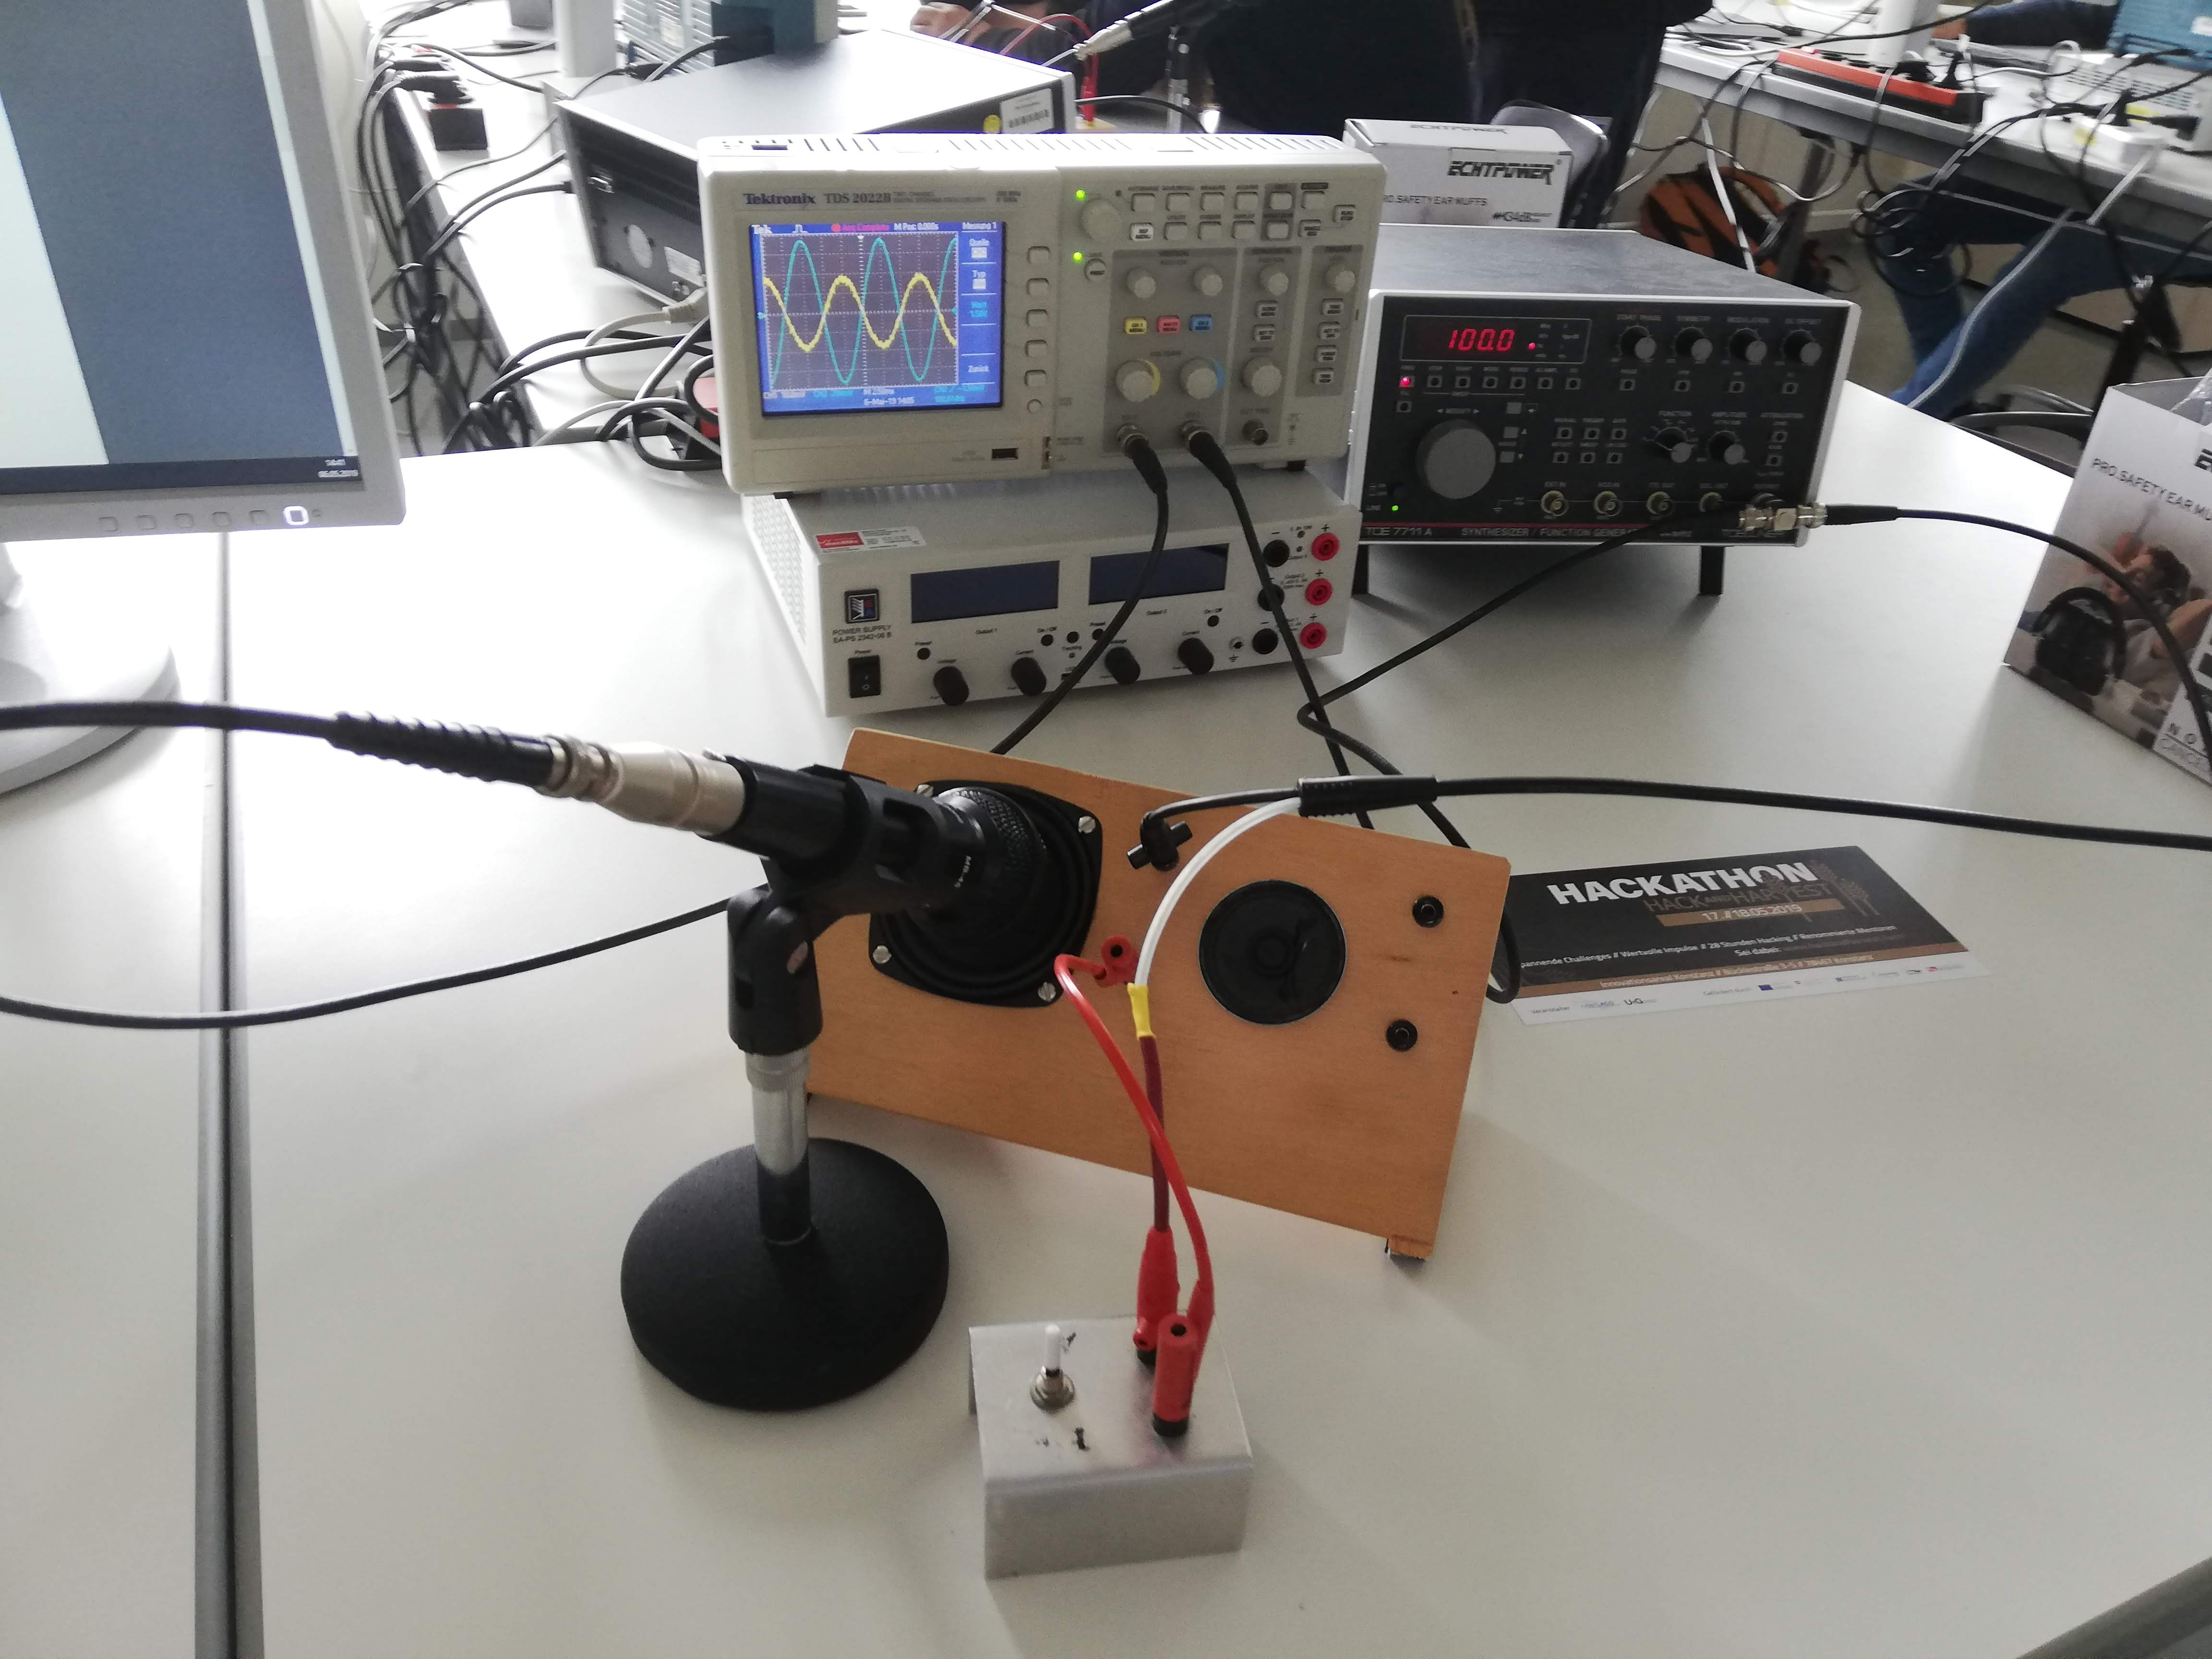
\includegraphics[width=0.6\textwidth]{media/aufbau.jpg}
	\caption{Aufbau im Labor}
	\label{fig:Aufbau im Labor}
\end{figure}
\newpage
\section{Messwerte}
\label{chap:VERSUCH_1_MESSWERTE}

Durch die Kalibrierung im Skript und die Justierung der Geräte und des Grauwertkeils haben wir ein Bild dessen gemacht.

\begin{figure}[hbt!]
	\centering\small
	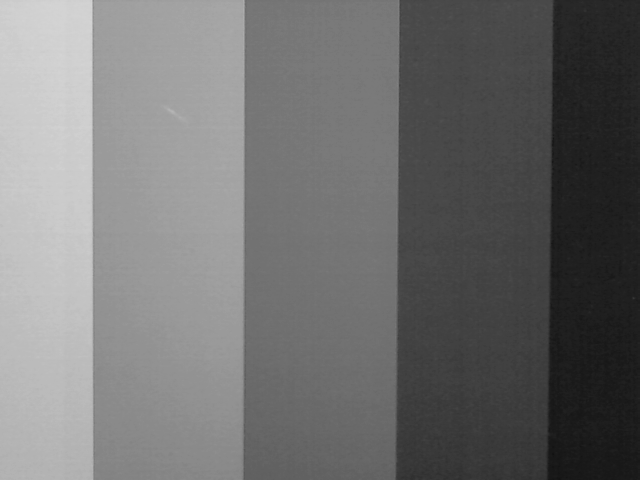
\includegraphics[width=0.5\textwidth]{../data/Versuch1a.png}
	\caption{Das Bild des Grauwertkeiles}
	\label{fig:Das Bild des Grauwertkeiles}
\end{figure}
\label{chap:VERSUCH_2_MESSWERTE_TABELLE}
Tabelle [\ref{chap:VERSUCH_2_MESSWERTE_TABELLE}] zeigt die Kalibrierungen, die wir vorgenommen haben, dass die Kamera stets die selben Werte hat.
Dies wurde mit \textit{.set(3, 640)}. Dabei wird im ersten Teil, hier als 3 definiert die Einstellung gesucht. In diesem Fall die Frame Breite. Im zweiten Teil wird die Frame Breite definiert. Hier als 640 Pixel.

\begin{table}[H]
	\centering\small
	\begin{tabular}{|c|c|c|}
		\hline
		\textbf{Beschreibung} & \textbf{Wert} & \textbf{Wertebereich} \\
		\hline
		Frame Width & 640 & Je nach Bedarf  \\
		\hline
		Frame Height & 480 & Je nach Bedarf  \\
		\hline
		Brightness & 133 & 0 - 255  \\
		\hline
		Contrast & 32 & 0 - 255  \\
		\hline
		Saturation & 32 & 0 - 255 \\
		\hline
		Gain & 20 & 0 - 255  \\
		\hline
		Exposure & -4 & -1 - -7 \\
		\hline
		White Balance & 10000 & 0 - 10000  \\
		\hline
	\end{tabular}
	\caption{Messwerte Kalibrierung}
	\label{fig:VERSUCH_1_MESSWERTE_TABELLE}
\end{table}

\newpage
\section{Auswertung}
\label{chap:VERSUCH_1_AUSWERTUNG}
Da das Bild einen starken Blaustich hat, haben wir die Datei im Nachhinein mit 
\newline 
\textit{cv2.IMREAD\_GRAYSCALE} in Schwarz Weiß gefärbt.
In den folgenden Abbildung sind die einzelnen Aufteilungen vom Bild des Grauwertkeils dargestellt.
Hierfür wurde zuerst in der Python Datei \textit{task1.2} mit der Pythonbibliothek \textit{cv2} das Bild des Grauwertkeils mit manuellen Grenzwerten in ihre einzelnen Grauwerte aufgeteilt.
Die Dateien (a) bis (e) sind die einzelnen Grauwerte. (f) ist das gesamte Bild des Grauwertkeils.
\begin{figure}[hbt!]
  	\centering
  	\subfloat[Grauwert1]{
		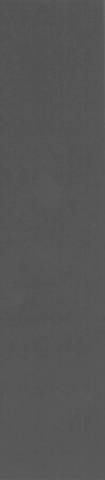
\includegraphics[width=0.08\textwidth]{../data/bild1.png}\label{fig:f1}}
  	\subfloat[Grauwert2]{
		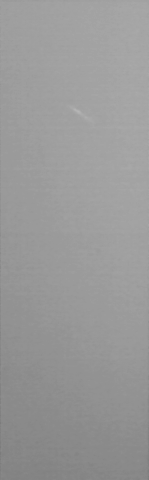
\includegraphics[width=0.08\textwidth]{../data/bild2.png}\label{fig:f2}}
  	\subfloat[Grauwert3]{
		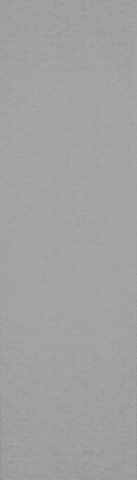
\includegraphics[width=0.08\textwidth]{../data/bild3.png}\label{fig:f3}}
  	\subfloat[Grauwert4]{
		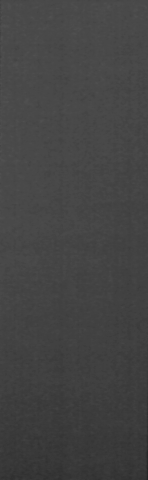
\includegraphics[width=0.08\textwidth]{../data/bild4.png}\label{fig:f4}}
  	\subfloat[Grauwert5]{
		
\includegraphics[width=0.08\textwidth]{../data/bild5.png}\label{fig:f5}}
		\hfill
	\subfloat[Grauwertkeil]{
		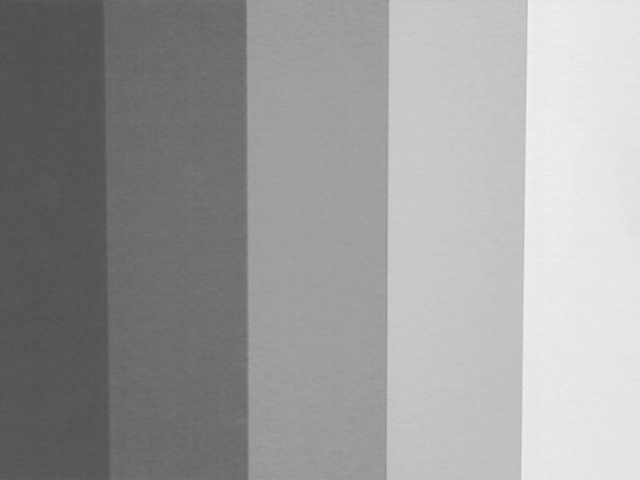
\includegraphics[width=0.4 \textwidth]{../data/Versuch1b.png}\label{fig:f6}}
	\caption{Die einzelnen Grauwerte und das zusätzliche Gesamtbild}
\end{figure}
\newpage
Mittels \textit{cv2.mean()} haben wir nun den den durchschnittlichen Grauwert der einzelnen Graustufen berechnet und mit \textit{np.std()} die Standartabweichung.
Zudem haben wir den Hexwert mit matplotlib berechnet. Das Ganze haben wir so in die Konsole ausgegeben, dass wir direkt den Konsolenoutput in LaTeX einfügen konnten.
Die Tabelle ist bei den Messergebnissen Tabelle 2.2 einsehbar.

Tabelle [\ref{chap:VERSUCH_3_MESSWERTE}] zeigt die in Python berechneten Werte für die einzelnen Graustufen die einzelnen Grauwerte, den Hexwert, sowie die Standardabweichung 

\begin{table}[H]
	\centering\small
	\begin{tabular}{|c|c|c|c|c|c|}
		\hline
		Graustufe & Grauwert & Hex-Value & Standartabweichung \\
		\hline
		Graustufe 1 & 86.39761904761905 &  \#161616 & 2.082341260388545 \\
		\hline
		Graustufe 2 & 112.00498456790123 &  \#1d1d1d & 2.6116529874626044 \\
		\hline
		Graustufe 3 & 161.2048205596107 &  \#292929 & 2.2861194924984116 \\
		\hline
		Graustufe 4 & 199.60105744949496 &  \#333333 & 2.968662423351764 \\
		\hline
		Graustufe 5 & 235.58106563421828 &  \#3c3c3c & 2.582844019720398 \\
		\hline
	\end{tabular}
	\caption{Grauwert, Hexwert und Standardabweichung für die einzelnen Grauwerte}
	\label{fig:VERSUCH_3_MESSWERTE}
\end{table}



\newpage
\section{Interpretation}
\label{chap:VERSUCH_1_INTERPRETATION}
Durch einen Messfehler ist der Grauwertkeil in farbig statt in Schwarz Weiß aufgenommen worden. 
Dies haben wir durch die Funktion \textit{cv2.IMREAD\_GRAYSCALE} behoben. Die einzelnen Abschnitte der Grauwerte sind ungleich hoch, da die einzelnen Grauwerte nicht alle parallel nach unten verlaufen und sonst noch Pixel von anderen Grauwerten beinhalten würden.
\newline
Die Werte auf der y-Achse sind die Grauwerte in RGB, während die x-Achse den Grauwertkeil von 1 bis 5 darstellt.
Der Grauwert könnte von 0 für schwarz bis 255 für weiß gehen.
\newline
Die Ausschwenkung des zweiten Grauwertes könnte daran liegen, dass dunkle Farben durch Sensorrauschen und seitlichen Lichteinfluss dunkler wirken, als sie tatsächlich sind.
Eine andere Theorie ist, dass die Grauwerte auf dem Keil nicht linear dunkel sind, sondern der Grauwert einfach dunkler ist als im Schnitt.
So hat der zweite Wert die zweitgröte Standartabweichung sämtlicher Grauwerte.
\newline
Im Gesamten kann man aber sagen, dass die Farben eine relativ geringe Standardabweichung haben die in RGB-Werten zwischen 2,08 und 2,96 liegt.
\begin{figure}[hbt!]
  	\centering
  	\subfloat[Durchschnittlicher Grauwert]{
		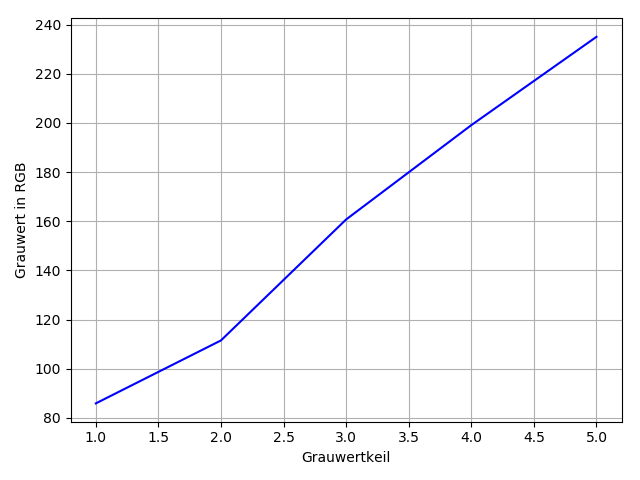
\includegraphics[width=0.45\textwidth]{media/myplot.png}\label{fig:f1}}
	\hfill
  	\subfloat[Standardabweichung des Grauwerts]{
		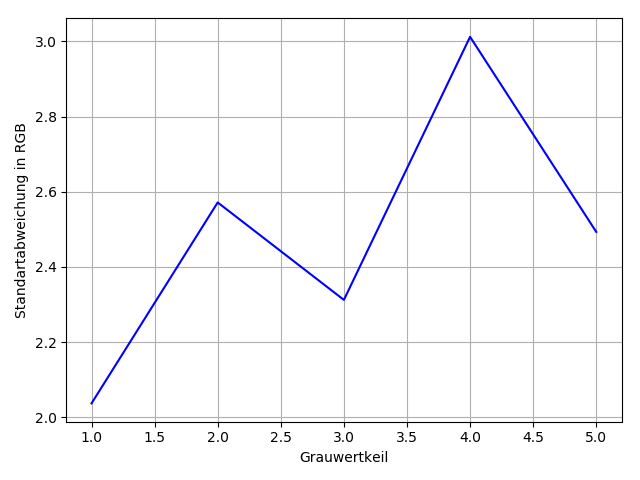
\includegraphics[width=0.45\textwidth]{media/myplot2.png}\label{fig:f2}}
	\caption{Standardabweichung und Durchschnitt der jewiligen Grauwerte}
\end{figure}

%
% CHAPTER Versuch 2
%
\chapter{Versuch 2: Aufnahme eines Dunkelbildes}
\label{chap:VERSUCH_2}

\section{Fragestellung, Messprinzip, Aufbau, Messmittel}
\label{chap:VERSUCH_2_FRAGESTELLUNG}
Im Versuch 2 sollten wir die Kamera so abdecken, dass das Bild komplett schwarz erscheint. Dies haben wir mit einem schwarzen Mousepad gemacht.
Mit den selben Kameraeinstellungen wie bei der Aufnahme des Grauwertkeils sollten wir nun 10 Bilder machen. 
\newline
Dies haben wir in Python mit einer simplen for-Schleife verwirklicht.
Danach sollten wir wieder in Python die 10 Bilder einlesen, in \textit{double} umwandeln und den pixelweisen Mittelwert berechnen.
\newline
\newline
Da die Webcam standartmäßig nur Farbbilder liefert, müssen wir noch die Bilder in Grauwertbilder umwandeln.
Da man nun 307200 Mittelwerte für den Durchschnitt der 10 Bilder erhält, speichern wir diese in einem Vektor um die for-Schleife effizienter zu machen.
\newline
Aus den sämtlichen Mittelwerten wiederrum, haben wir uns ein Bild erstellen lassen und dieses kontrastmaximiert dargestellt.
Danach haben wir von jedem Pixel im Grauwertkeil den entsprechenden Mittelwertspixel abgezogen. Dieses korrigierte Bild wurde daraufhin gespeichert.


\newpage
\section{Messwerte}
\label{chap:VERSUCH_2_MESSWERTE}
Hier ist eines der 10 aufgenommenen Dunkelbilder, die durch das Pythonskript gecaptured wurden.
\begin{figure}[hbt!]
	\centering\small
	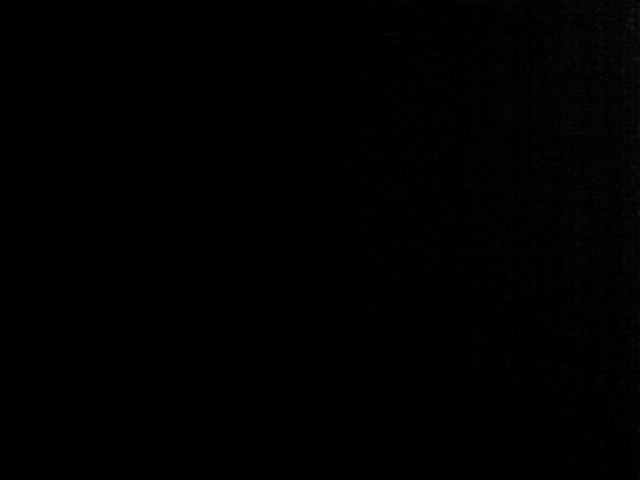
\includegraphics[width=0.9\textwidth]{../data/black1.png}
	\caption{Eines der 10 aufgenommenen Dunkelbilder}
	\label{fig:Eines der 10 aufgenommenen Dunkelbilder}
\end{figure}
\newpage
\section{Auswertung}
\label{chap:VERSUCH_2_AUSWERTUNG}
Um die Webcam abzudecken, haben wir das im Labor für die PC's verwendete Mousepad genommen.
Mit der Funktion \textit{cv2.equalizeHist(image)} erhalten wir ein kontrastmaximiertes Bild. Dieses ist in der Abbildung 3.2 einsehbar.
Das Bild hat einen konstanten Grauwert von 71.
\begin{figure}[hbt!]
	\centering
  	\subfloat[Aufnahme des Grauwertkeils]{
		
\includegraphics[width=0.45\textwidth]{../data/blackaverage.png}\label{fig:f1}}
	\hfill
	\subfloat[kontrastmaximiertes Bild]{
		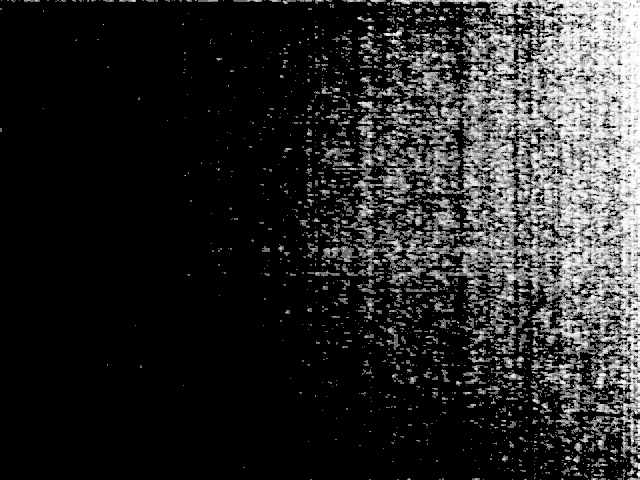
\includegraphics[width=0.45\textwidth]{../data/contrastblackaverage.png}\label{fig:f2}}
	\caption{Grauwertkeil und kontrastmaximiertes Bild}
\end{figure}

Nachdem wir das Bild des pixelweisen Durchschnittes und das Bild des Grauwertkeils eingelesen haben und in ein Schwarz-Weiß Bild umgewandelt haben, subtrahieren wir vom Bild des Grauwertkeiles das Bild des pixelweisen Durchschnittes.
Dabei erhalten wir die Abbildung in 3.2.b.


\begin{figure}[hbt!]
  	\centering
  	\subfloat[Aufnahme des Grauwertkeils]{
		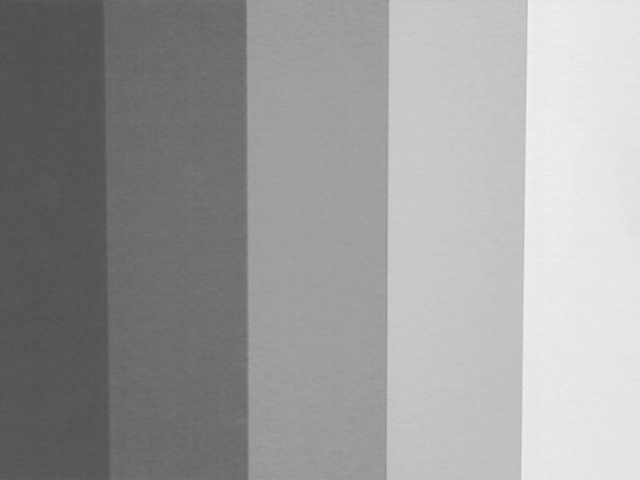
\includegraphics[width=0.45\textwidth]{../data/Versuch1b.png}\label{fig:f1}}
	\hfill
  	\subfloat[Korrigiertes Bild]{
		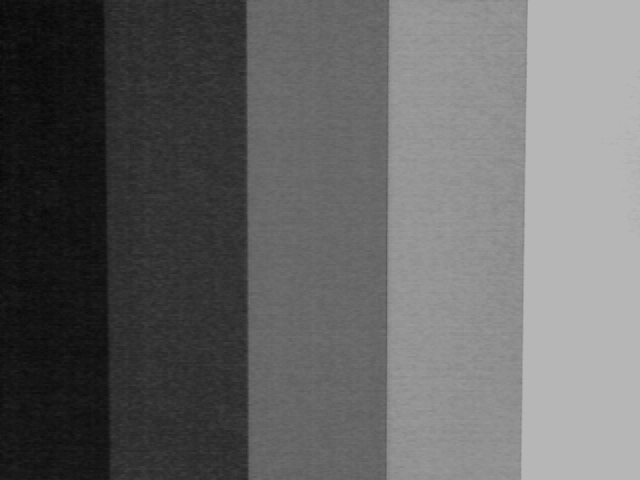
\includegraphics[width=0.45\textwidth]{../data/korrigiertes_bild.png}\label{fig:f2}}
	\caption{Unterschied zwischen dem richtigen und dem korrigerten Bild}
\end{figure}

\newpage
\section{Interpretation}
\label{chap:VERSUCH_2_INTERPRETATION}
Da das kontrastmaximierte Bild keine Veränderungen aufweist im Vergleich zum normalen Durchschnittsbild wissen wir, dass es keine Kontraste gibt und das Bild überall dieselbe Farbe besitzt.
Das Bild hat nicht den Grauwert 0 sondern 71, da wir die Belichtungseinstellungen von dem Bild des Grauwertkeiles verwendet haben.
\newline
Aufgrunddessen haben wir die Gewissheit, dass wir die Kamera vollständig abgedeckt haben, ohne dass es einen externen Lichteinfluss gab.
Schlichtweg würde das kontrastmaximierte Bild darstellen,  dass es keine Störfaktoren in der Webcam gibt und alle denselben Nullpunkt haben.
\newline
\newline
Durch die Subtraktion des durchschnittlichen Dunkelbildes, erhalten wir den Nullpunkt jedes einzelnen Pixels. Durch diesen Vorgang könnten wir theoretisch das thermische Rauschen entfernen.
Da unser durchschnittliches Dunkelbild keine Unterschiede aufweist, wissen wir jedoch, dass es kein thermisches Rauschen gibt.
%
% CHAPTER Versuch 3
%
\chapter{Versuch 3: Aufnahme eines Weißbildes}
\label{chap:VERSUCH_3}

\section{Fragestellung, Messprinzip, Aufbau, Messmittel}
\label{chap:VERSUCH_3_FRAGESTELLUNG}
Im dritten Versuch nehmen wir ein weißes Blatt Papier und legen dieses auf den Grauwertkeil. Dadurch haben wir den selben Abstand wie zum Grauwertkeil.
Dabei wird die Belichtung auf 30-50\% der Hellsättigung eingestellt.
\newline
Hierbei sollten keine Schatten oder andere Störfaktoren auftreten.
Auch hier nehmen wir mit unserem Programm 10 Bilder auf.
\newline
Mittels einem Pythonskript berechnen wir daraufhin den Mittelwert jedes einzelnen Pixels. Durch den Mittelwert elimieren wir das thermische Rauschen.
Von den Mittelwerten des weißen Bildes werden wir das Dunkelbild abziehen und erhalten daraus das resultierende Weißbild.
Das Bild geben wir zudem kontrastmaximiert dar.
\newline
\newline
Das berechnete Weißbild wird nun normiert mit dem Mittelwert 1.
\newline
Der Grauwertkeil wird mit dem Dunkelbild subtrahiert und danach mit dem normierten Weißbild dividiert.
\newline
Durch das kontrastmaximierte Bild können wir nun so die Intensität des einfallenden Lichts betrachten.
\newpage
\section{Messwerte}
\label{chap:VERSUCH_3_MESSWERTE}
Hier ist eines der aufgenommen Bilder vom weißen Blatt Papier.
Leider ist durch einen Aufnahmefehler das Bild blau geworden. Dieses Problem haben wir durch das einlesen im Python Programm durch folgenden Code behoben:
\newline
\newline
\lstinputlisting[style=PYTHON, frame=single, label=lst:APPENDIX_SOURCECODE_AREA5]{../grayscale.py}
\newline
\newline 
Durch \textit{cv2.IMREAD\_GRAYSCALE} wird das Bild in ein Schwarz-Weiß Bild umgewandelt.
\newline
\newline
\begin{figure}[hbt!]
	\centering\small
	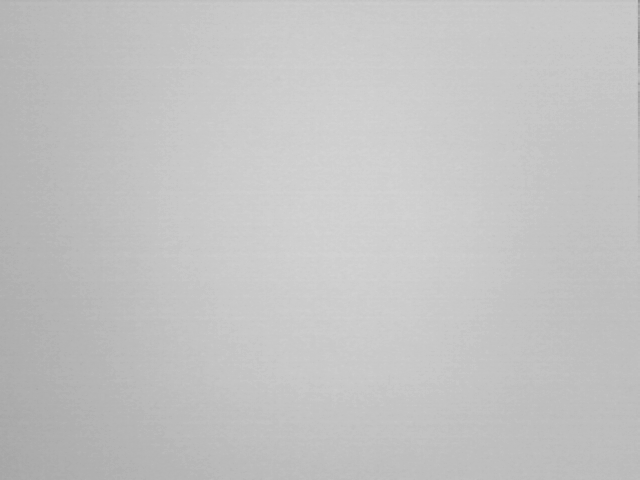
\includegraphics[width=0.9\textwidth]{../data/white1.png}
	\caption{Eines der 10 aufgenommenen Weißbilder}
	\label{fig:Eines der 10 aufgenommenen Weißbilder}
\end{figure}
\newpage
\section{Auswertung}
\label{chap:VERSUCH_3_AUSWERTUNG}
Nun haben wir in zwei for-Schleifen für jeden Pixel den Durchschnitt aller 10 Bilder ausgewertet und in ein neues Bild geschrieben.
Das untenstehende linke Bild zeigt den Pixelweisen Durchschnitt. 
Das rechte der beiden Bilder ist das linke Bild kontrastmaximiert.

\begin{figure}[hbt!]
	\centering
  	\subfloat[Pixelweiser Mittelwert der einzelnen Bilder]{
		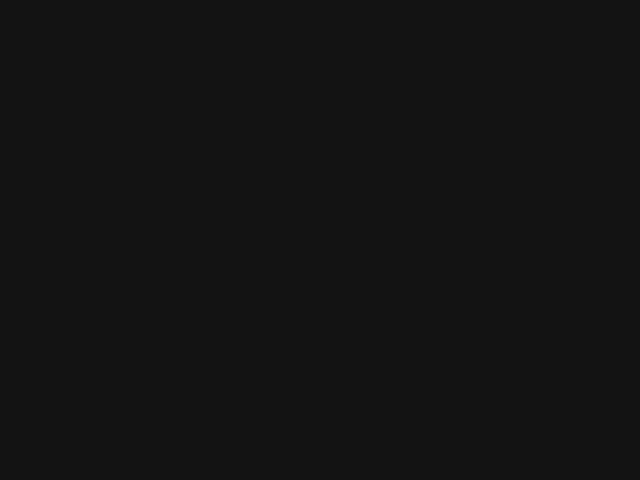
\includegraphics[width=0.45\textwidth]{../data/whiteaverage.png}\label{fig:f1}}
	\hfill
	\subfloat[kontrastmaximiertes Bild der Weißbilder]{
		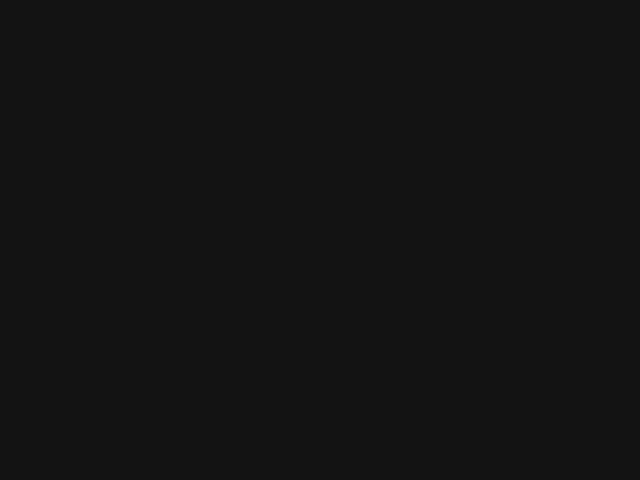
\includegraphics[width=0.45\textwidth]{../data/contrastwhiteaverage1.png}\label{fig:f2}}
	\caption{Mittelwert der Weißbilder und kontrastmaximiertes Bild}
\end{figure}

Um die tatsächliche Intensität des Lichtes zu bestimmen und die Sensitivitäten der einzelnen Pixel, mussten wir zuerst das das Weißbild mit dem Dunkelbild subtrahieren.

\begin{figure}[hbt!]
	\centering\small
	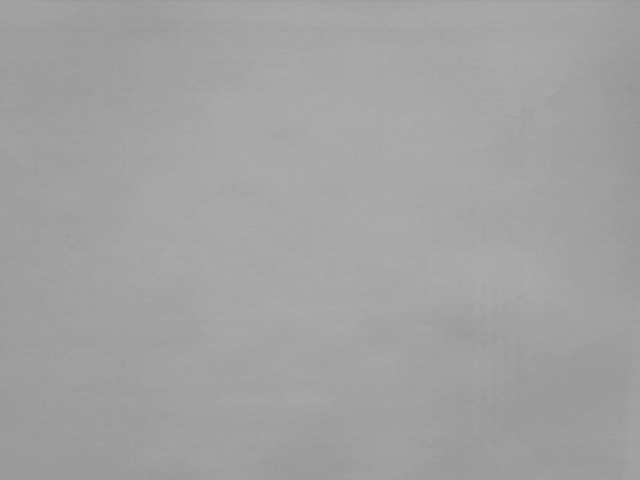
\includegraphics[width=0.7\textwidth]{../data/whiteminusblack.png}
	\caption{Dunkelbild subtrahiert vom Weißbild}
	\label{fig:Dunkelbild subtrahiert vom Weißbild}
\end{figure}

\newpage
Danach war es die Aufgabe das Weißbild zu normieren, dass der Mittelwert 1 ist. Das durch Abzug des Dunkelbildes korrigierte Eingangsbild wird anschliessend durch das normierte Weißbild dividiert.

\begin{figure}[hbt!]
  	\centering
  	\subfloat[Grauwertkeil]{
		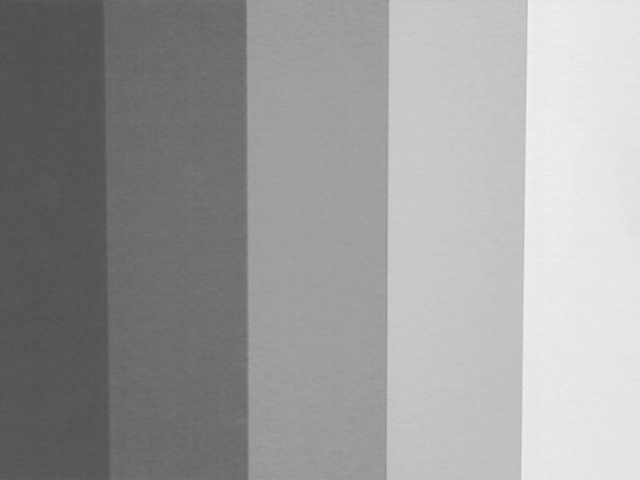
\includegraphics[width=0.45\textwidth]{../data/Versuch1b.png}\label{fig:f1}}
	\hfill
  	\subfloat[Bild mit der Intensität des Lichteinfalles]{
		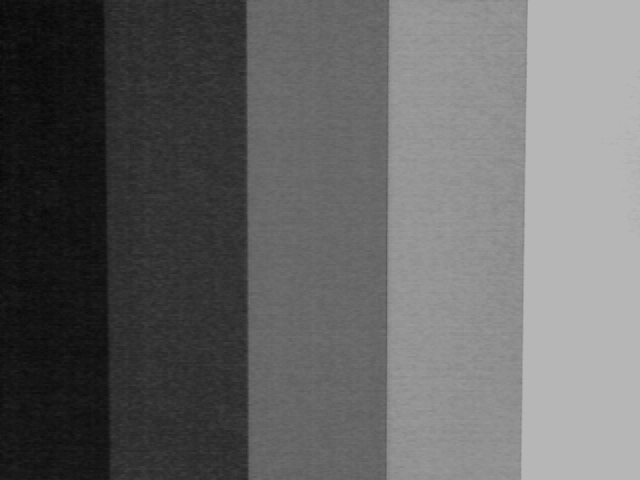
\includegraphics[width=0.45\textwidth]{../data/korrigiertes_bild2.png}\label{fig:f2}}
	\caption{Unterschied zwischen dem Grauwertkeil und dem Bild mit der Intensität des Lichteinfalles}
\end{figure}
\newpage
\section{Interpretation}
\label{chap:VERSUCH_3_INTERPRETATION}
Das Bild hat ebenfalls wie die Aufnahme des Grauwertkeils einen starken Blautstich.
Dies haben wir gelöst durch eine Konvertierung ins Blaue. 
\newline
Bei der Auswertung haben wir das kontrastmaximierte Bild neben dem des durchschnittlichen Weißbildes, 
sieht man schön die Verstärkung.
Hier sieht man eine Vignettierung des Bildes d.h. die Optik der Kamera
übeträgt die Helligkeit nicht gleichmäßig auf den Sensor.
\newline
\newline
Dies wird sichtbar durch eine Abdunkelung des Bildes zu den Rändern hin.
Nachdem man Weißbild minus Dunkelbild berechnet hat, bekommt man ein dunkleres Weißbild, bei dem man immer noch leicht die Vignettierung beobachten kann.
\newline
\newline
In dem letzten Experiment wurde die Intensität des einfallenden Lichtes berechnet.
In schwarz kann man nun gut betrachten, wie das Licht eingefallen ist.
\newline
Die Kamera war auf ihrer Halterung so zum Fenster gerichtet, dass das Licht von oben eingefallen ist.
\newline
Auch hier ist wieder eine Art Vignettierung zu sehen in weiß.
Der Lichteinfall stimmt auch mit dem kontrastmaximierten Bild von vorher überin, da am oberen Teil des Bildes die Vignettierung nicht so stark ist bzw. das Licht von oben einfällt.


%
% CHAPTER Versuch 4
%
\chapter{Versuch 4: Aufnahme eines Weißbildes}
\label{chap:VERSUCH_4}

\section{Fragestellung, Messprinzip, Aufbau, Messmittel}
\label{chap:VERSUCH_4_FRAGESTELLUNG}
Im vierten Versuch war es die Aufgabe funktionsuntüchtige Pixel, wie zum Beispiel Hot, Stuck und Deadpixel zu entdecken und zu markieren.
Deadpixels sind Pixel die immer auf ihrem niedrigsten Wert steckenbleiben.
\newline 
Stuck Pixels bleiben immer auf ihrem höchsten Wert, während Hot Pixels in die Sättigung gehen bei längeren Belichtungszeiten.
Zudem sollen wir mithilfe des Programmes aus Aufgabe 3 das Bild des Grauwertkeiles korrigieren und es speichern.
\newline
\newline
Dies haben wir jedoch bereits schon in Aufgabe 3 gelöst. 
Danach sollten wir mit dem korrigierten Bild so verfahren wie in Aufgabe 1, indem wir das Bild mit den selben Einstellungen wie in Aufgabe 1 das Bild in 5 Unterbilder aufteilen und den durchschnittlichen Grauwert, den Hexwert und die Standartabweichung berechnen.
\newline
Diesen werden wir im späteren Verlauf noch mit den Messungen aus Aufgabe 1 vergleichen.

\newpage
\section{Messwerte}
\label{chap:VERSUCH_4_MESSWERTE}

In der unteren Abbildung untersuchen wir ein Weißbild auf funktionsuntüchtige Pixel.
\begin{figure}[hbt!]
	\centering\small
	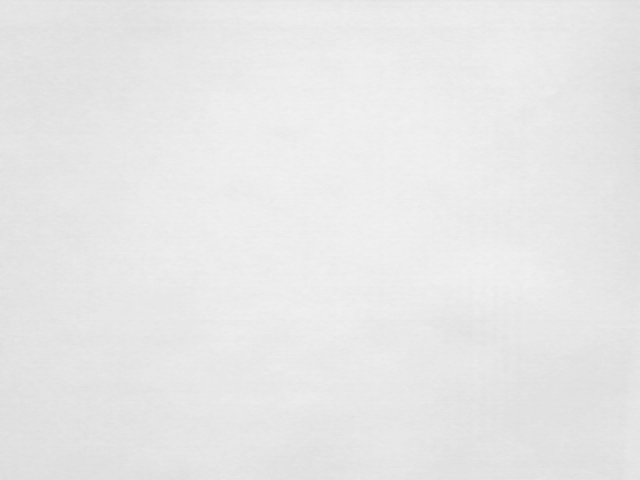
\includegraphics[width=0.7\textwidth]{../data/zzz.png}
	\caption{Weißbild mit Dead- und Stuckpixel}
	\label{fig:Weißbild mit Dead- und Stuckpixel}
\end{figure}

In der unteren Abbildung untersuchen wir ein Dunkelbild auf funktionsuntüchtige Pixel.

\begin{figure}[hbt!]
	\centering\small
	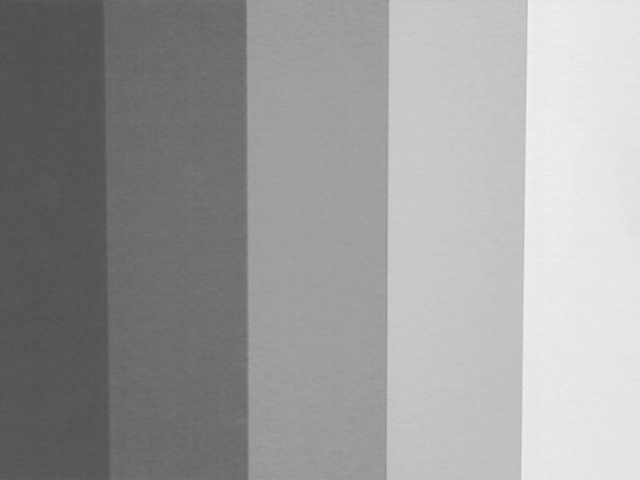
\includegraphics[width=0.7\textwidth]{../data/zzz2.png}
	\caption{Dunkelbild mit Dead- und Stuckpixel}
	\label{fig:Dunkelbild mit Dead- und Stuckpixel}
\end{figure}
\newpage
\section{Auswertung}
\label{chap:VERSUCH_4_AUSWERTUNG}

Mittels der OpenCV Bibliothek und der damit verbundenen Funktion \textit{cv2.circle} haben wir einen Kreis gezeichnet.
Mittels einer For-Schleife werden alle 307200 Pixel untersucht auf den dunkelsten und den hellsten Punkt. 
\begin{figure}[hbt!]
  	\centering
  	\subfloat[Weißbild mit dem dunkelsten Punkt]{
		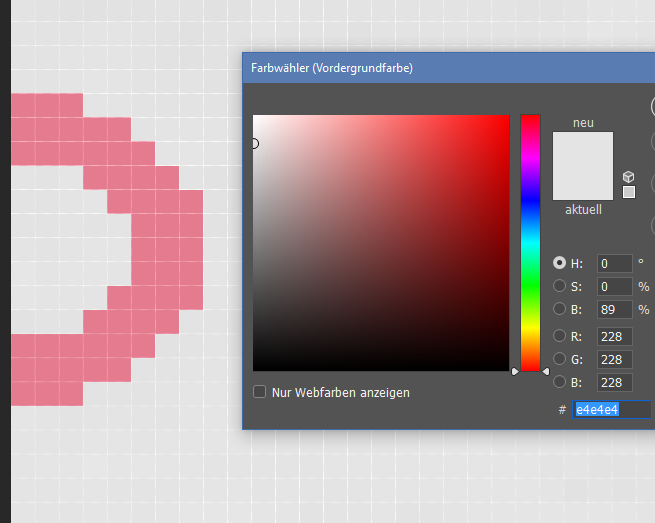
\includegraphics[width=0.45\textwidth]{../data/proof1.png}\label{fig:f1}}
	\hfill
  	\subfloat[Weißbild mit dem hellsten Punkt]{
		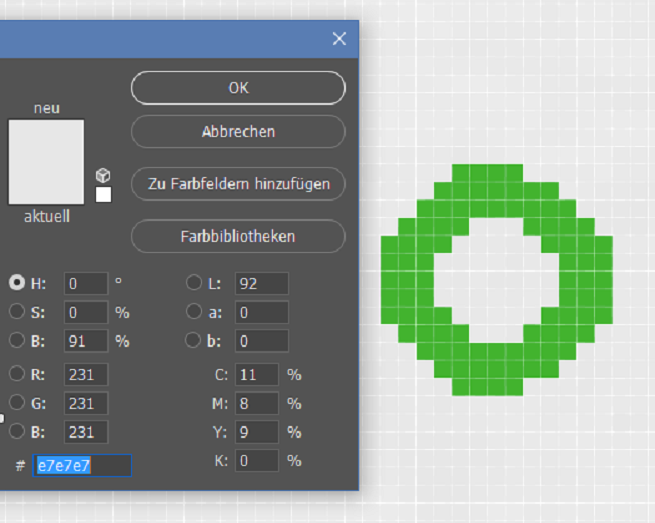
\includegraphics[width=0.45\textwidth]{../data/proof2.png}\label{fig:f2}}
	\caption{Unterschied zwischen dem hellsten und dem dunkelsten Bild}
\end{figure}
Das Dunkelbild wurde ebenfalls mit der Funktion \textit{cv2.circle} bearbeitet. Das Ergebnis sehen sie in der Abbildung 5.4.
\begin{figure}[hbt!]
	\centering\small
	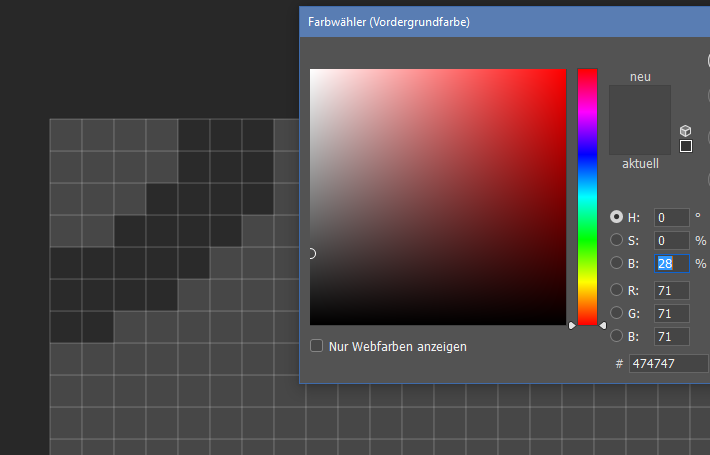
\includegraphics[width=0.5\textwidth]{../data/proof3.png}
	\caption{Dunkelbild mit Dead- und Stuckpixel}
	\label{fig:Dunkelbild mit Dead- und Stuckpixel}
\end{figure}
\newpage
Der mit dem normierten Weißbild korrigierte Graukeil, wird nochmal mit dem Skript aus der ersten Aufgabe berechnet.
In dieser Tabelle ist der Mittelwert, der HexValue und die Standardabweichung für die Intensität des Lichteinfalls.
\begin{table}[H]
	\centering\small
	\begin{tabular}{|c|c|c|c|}
	\hline
	Stufe & Mittelwert & Hex-Value & Standartabweichung \\
	\hline
	Stufe 1 & 241.67111111111112 & \#3e3e3e & 36.794374014010515 \\
	\hline
	Stufe 2 & 123.12765432098767 & \#1f1f1f & 101.62025094391961 \\
	\hline
	Stufe 3 & 60.187013381995136 & \#0f0f0f & 73.25401533025126 \\
	\hline
	Stufe 4 & 93.80972222222222 & \#181818 & 83.6389175516743 \\
	\hline
	Stufe 5 & 160.29564564564564 & \#292929 & 78.10787025296499 \\
	\hline
	\end{tabular}
	\caption{Mittelwert, Hexwert und Standardabweichung für die Intensivität des Lichteinfalls}
	\label{fig:VERSUCH_4_MESSWERTE}
\end{table}

\newpage
\section{Interpretation}
\label{chap:VERSUCH_4_INTERPRETATION}
Um die beiden Extrempunkte wurde ein roter Kreis um den dunkelsten Punkt gezeichnet und ein grüner Kreis um den hellsten Punkt.
Da weder 228 ein sehr dunkler Punkt ist noch 231 ein extrem weißer außergewöhnlicher Punkt ist im Bild, gibt es im Weißbild weder Stuck-, noch Deadpixels.
Auch das Dunkelbild weißt keine Dead- oder Stuckpixels auf.
Das gesamte Bild hat einen durchgehenden Grauwert von 71.
So ist sowohl der höchste als auch der kleinste Farbwert bei 71.
\newline
\newline
Das korrigierte Bild mit dem Programm aus Aufgabe 3 wurde bereits in dem dritten Versuch gelöst und ausgewertet.
\newline
\newline
Da das Licht von oben in den Sensor der Kamera eingetreten ist, ist wie zu erwarten eine 'U' Form zu sehen.
Der Wert im dritten Graukeil ist am niedrigsten in der Abbildung 5.5.a, da dieser auch am meisten Schwarz Anteil hat.
Links und rechts davon steigt der Wert wieder an, durch die Vignettierung und den unterschiedlichen Lichteinfall. 
Die Standartabweichung ist wie zu erwarten beim zweiten und vierten Wert am höchsten, da diese wie in der Abbildung 4.4.b einen hohen Lichteinfall haben, aber trotzdem durch die Vignettierung eine nicht gleichmäßige Verteilung auf den Kamerasensor geschieht.
Der erste Wert hat die geringste Standartabweichung da dieser am meisten von dem Lichteinfall entfernt ist. 
\begin{figure}[hbt!]
  	\centering
  	\subfloat[Durchschnitt der Intensität des Lichteinfalls]{
		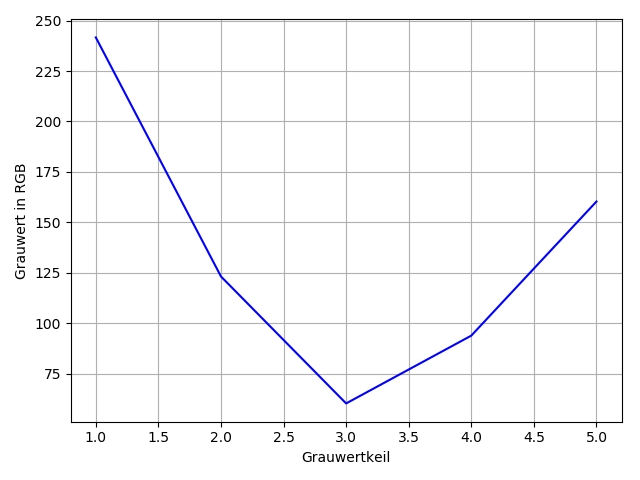
\includegraphics[width=0.45\textwidth]{../data/table1.png}\label{fig:f1}}
	\hfill
  	\subfloat[Standartabweichung der Intensität des Lichteinfalls]{
		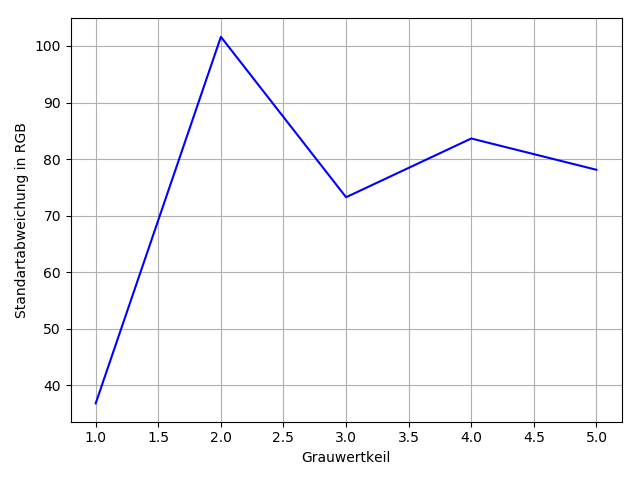
\includegraphics[width=0.45\textwidth]{../data/table2.png}\label{fig:f2}}
	\caption{Unterschied zwischen dem [Durchschnitt und der Standartabweichung der Intensität des Lichteinfalls}
\end{figure}

%
% CHAPTER Anhang
%
\renewcommand\thesection{A.\arabic{section}}
\renewcommand\thesubsection{\thesection.\arabic{subsection}}

\chapter*{Anhang}
\label{chap:APPENDIX}
\addcontentsline{toc}{chapter}{Anhang}
%\setcounter{chapter}{0}
\addtocounter{chapter}{1}
\setcounter{section}{0}

\section{Quellcode}
\label{chap:APPENDIX_SOURCECODE}

\subsection{Quellcode Versuch 1}
\label{chap:APPENDIX_SOURCECODE_V1}
\lstinputlisting[style=PYTHON, frame=single, caption=Bild einlesen von der Webcam und Bildeinstellungen, captionpos=b, label=lst:APPENDIX_SOURCECODE_MEASURE]{../task1.1.py}
\lstinputlisting[style=PYTHON, frame=single, caption=Bild in Grauwerte aufteilen, captionpos=b, label=lst:APPENDIX_SOURCECODE_MEASURE]{../task1.2.py}
\newpage
\lstinputlisting[style=PYTHON, frame=single, caption=LaTeX Tabelle mit Mittelwert\, Hexwert und Standartabweichung, captionpos=b, label=lst:APPENDIX_SOURCECODE_MEASURE]{../task1.3.py}
\newpage
\subsection{Quellcode Versuch 2}
\label{chap:APPENDIX_SOURCECODE_V2}
\lstinputlisting[style=PYTHON, frame=single, caption=Pixelweisen Mittelwert der 10 Dunkelbilder berechnen und Bild ausgeben, captionpos=b, label=lst:APPENDIX_SOURCECODE_REGRESSION]{../task2.1.py}
\newpage
\lstinputlisting[style=PYTHON, frame=single, caption=Bild vom Grauwertkeil vom Dunkelbild abziehen, captionpos=b, label=lst:APPENDIX_SOURCECODE_REGRESSION]{../task2.2.py}
\newpage
\subsection{Quellcode Versuch 3}
\label{chap:APPENDIX_SOURCECODE_V3}
\lstinputlisting[style=PYTHON, frame=single, caption=Pixelweisen Mittelwert der 10 Weißbilder berechnen und Bild ausgeben, captionpos=b, label=lst:APPENDIX_SOURCECODE_AREA1]{../task3.1.py}
\newpage
\lstinputlisting[style=PYTHON, frame=single, caption=Das berechnete Weißbild minus das Dunkelbild, captionpos=b, label=lst:APPENDIX_SOURCECODE_AREA2]{../task3.2.py}
\lstinputlisting[style=PYTHON, frame=single, caption=Bild normieren, captionpos=b, label=lst:APPENDIX_SOURCECODE_AREA3]{../task3.3.py}
\lstinputlisting[style=PYTHON, frame=single, caption=korrigiertes Bild erneut aufteilen in die einzelnen Grauwerte, captionpos=b, label=lst:APPENDIX_SOURCECODE_AREA4]{../task3.4.py}
\lstinputlisting[style=PYTHON, frame=single, caption=Mittelwert\, Hexwert und Standartabweichung berechnen, captionpos=b, label=lst:APPENDIX_SOURCECODE_AREA5]{../task3.4b.py}
\subsection{Quellcode Versuch 4}
\label{chap:APPENDIX_SOURCECODE_V4}
\lstinputlisting[style=PYTHON, frame=single, caption=Deadpixels berechnen, captionpos=b, label=lst:APPENDIX_SOURCECODE_AREA6]{../dead.py}
\newpage
\lstinputlisting[style=PYTHON, frame=single, caption=Stuckpixels berechnen, captionpos=b, label=lst:APPENDIX_SOURCECODE_AREA7]{../dead2.py}
\newpage
\section{Kameraeinstellungen für OpenCV}
\label{chap:APPENDIX_MEASUREMENT_SOURCE}
\begin{figure}[hbt!]
	\centering\small
	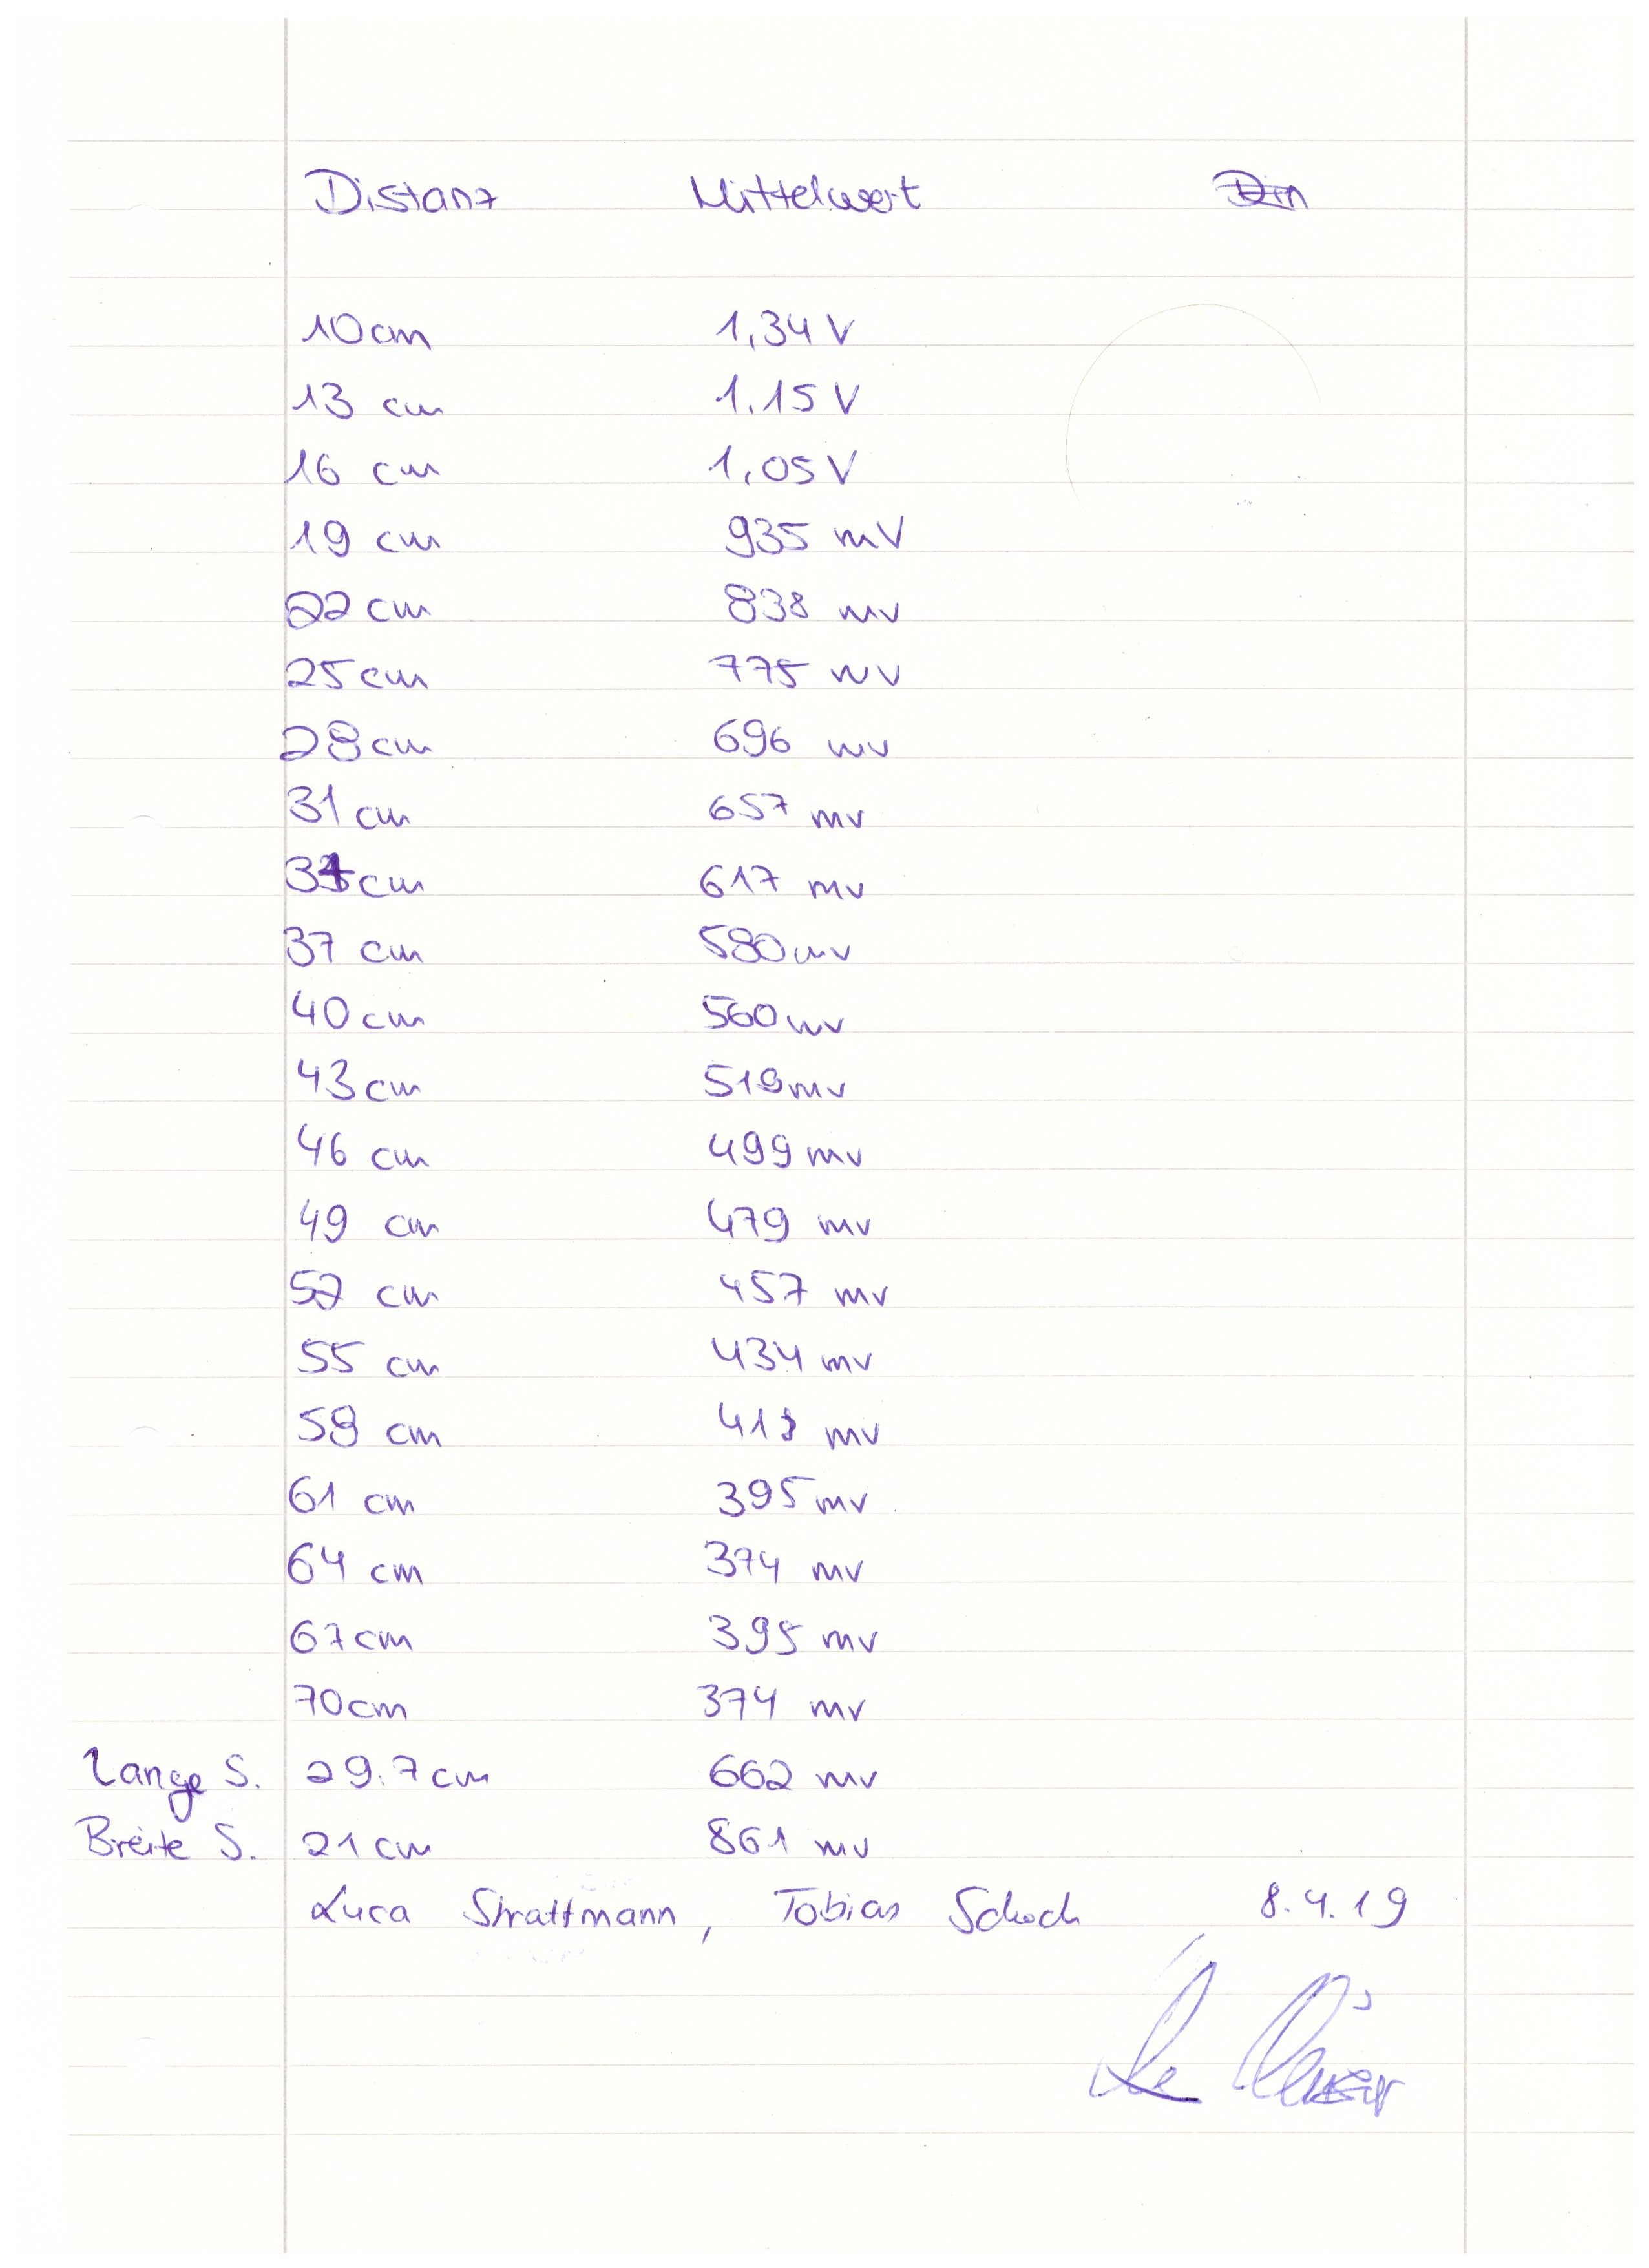
\includegraphics[width=0.8\textwidth]{media/scan.png}
	\caption{Kameraeinstellungen für OpenCV}
	\label{fig:Kameraeinstellungen für OpenCV}
\end{figure}

%
% Literaturverzeichnis
%
%\setcounter{chapter}{0}
\addtocounter{chapter}{1}
\setcounter{section}{1}

%
% Literaturverzeichnis
%
\phantomsection
\addcontentsline{toc}{chapter}{Literaturverzeichnis}
\bibliography{../references}
\newpage

\end{document}


\end{document}
%------------------------------------
% ╔═╗╔╗╔╔╦╗  ╔╦╗╔═╗╔═╗╦ ╦╔╦╗╔═╗╔╗╔╔╦╗
% ║╣ ║║║ ║║   ║║║ ║║  ║ ║║║║║╣ ║║║ ║ 
% ╚═╝╝╚╝═╩╝  ═╩╝╚═╝╚═╝╚═╝╩ ╩╚═╝╝╚╝ ╩ 
%------------------------------------